% !TeX encoding = UTF-8
% !TeX program = xelatex
% !TeX spellcheck = en_US
%
% 盲审版：在 main.tex 基础上去除封面、扉页、学术诚信声明、致谢。
% 其余内容与最终版 main.tex 保持一致。

\documentclass[
    fontset=fandol,
    degree=bachelor,
    pdf
]{sysuthesis}
% degree      = doctor | master | bachelor
% degree-type = academic | professional
% language    = chinese | english
% fontset     = windows | mac | ubuntu | fandol

% 加载宏包、全部的配置
\input{sysusetup.tex}

% 将超链接（含目录）颜色统一改为黑色，覆盖 sysuthesis.cls 中 pdf 选项下的默认 green
\hypersetup{allcolors=black}

% 盲审版：去除每页页眉的"中山大学本科毕业论文"标识及其上下横线
% 覆盖 sysuthesis.cls 中 plain 页面样式（line 1594-1604）以满足匿名要求
\makeatletter
\fancypagestyle{plain}{%
  \fancyhf{}%
  \fancyfoot[C]{\fontsize{9bp}{12bp}\selectfont\thepage}%
  \renewcommand\headrulewidth{0pt}%
  \let\@mkboth\@gobbletwo
  \let\chaptermark\@gobble
  \let\sectionmark\@gobble
}
\makeatother
\pagestyle{plain}

% 盲审版：覆盖 hyperref 的 PDF 元数据，清除作者姓名以满足匿名要求。
% sysuthesis 类在 \AtBeginDocument 中将 pdfauthor 设为 \sysu@author，
% 这里再注册一个 \AtBeginDocument 钩子以保证在其之后生效。
\AtBeginDocument{%
  \hypersetup{pdfauthor={},pdfsubject={},pdfkeywords={}}%
}

\begin{document}

% 盲审版：以下两行已注释，移除封面、扉页和学术诚信声明
% \maketitle
% \copyrightpage

\frontmatter
% !TeX root = ../main.tex

\sysusetup{
  keywords  = {细胞色素P450，酶底物特异性，EZSpecificity，图神经网络，泄漏控制外部评估},
  keywords* = {Cytochrome P450, Enzyme-substrate specificity, EZSpecificity, Graph neural network, Leakage-controlled external evaluation},
}

\begin{abstract}
  酶底物特异性预测是生物催化、合成生物学与药物研发中的核心任务。2025 年发表于 \textit{Nature} 的 EZSpecificity 模型是该任务的代表性先进方法，声称具有跨酶家族通用性；然而其训练数据集 ESIBank 在细胞色素 P450 超家族上覆盖稀缺（25{,}225 条酶中仅 389 个 P450，占 $1.5\%$），而 P450 在药物代谢、植物次生代谢与农药降解中应用价值重要，可作为检验该通用性的严格外部评估基准。本研究开展三方面工作：其一，针对现有 P450 数据库多数仅提供酶序列、或配体类型（底物/产物/抑制剂/辅因子）记录不明的普遍局限，通过文献检索、PDB 结构分析与多轮人工审核（辅以多智能体协作流程），对整合自 RCSB PDB、ESIBank、P450Rdb、PlantP450DB 与 PCPD 五个来源的每条酶--配体记录严格复核与分类，构建了目前规模最大、标注最详细的 P450 酶--底物特异性公开基准数据集，含 1{,}622 个酶、2{,}125 个底物、47{,}510 条可用样本（正 4{,}362 / 负 43{,}148），显著扩展植物 P450 数据覆盖；其二，以 InterPro 功能域识别 ESIBank 原始训练集中的 389 个 P450 并过滤测试集对应样本，建立泄漏控制的外部公平对比协议；其三，引入残基级几何向量感知（GVP）通路构成双图架构，以零初始化加延迟解冻保证基线等价。在 7{,}963 条过滤后测试集上，EZSpecificity 公开预训练模型 Test AUC $= 0.5586$、AUPR $= 0.1004$（接近 $1{:}10.2$ 正负比随机基线）；本研究领域专属基线达到 AUC $= 0.9205$、AUPR $= 0.6403$（$\Delta\mathrm{AUC} = +0.3619$）。双图架构在单随机切分下与基线相当（AUC $+0.0008$、AUPR $-0.0275$），未见显著收益。研究结果表明通用先进模型在训练集稀缺家族上存在明显的 未见酶的泛化瓶颈，领域专属数据重训可显著改善 P450 特异性预测表现。
\end{abstract}

\begin{abstract*}
  Enzyme--substrate specificity prediction is a core task in biocatalysis, synthetic biology, and drug discovery. EZSpecificity, a cross-attention graph neural network published in \textit{Nature} in 2025, is a leading state-of-the-art method that claims generality across diverse enzyme families. However, its training dataset ESIBank substantially under-represents the cytochrome P450 superfamily: only 389 P450 enzymes ($1.5\%$ of ESIBank's 25{,}225 total enzymes) are included, whereas P450s hold significant importance in drug metabolism, plant secondary metabolism, and pesticide degradation---making the family a rigorous external benchmark for testing the model's generality claim. This thesis pursues three lines of work. First, to address limitations of existing P450 databases---most provide only enzyme sequences or leave ligand types (substrate, product, inhibitor, cofactor) unspecified---each enzyme--ligand record integrated from RCSB PDB, ESIBank, P450Rdb, PlantP450DB, and PCPD was rigorously re-curated via literature retrieval, PDB structural analysis, and multi-round human review (assisted by a multi-agent collaboration pipeline). The resulting benchmark, to our knowledge currently the largest and most detailed public P450 enzyme--substrate specificity dataset, contains $1{,}622$ enzymes, $2{,}125$ substrates, and $47{,}510$ usable samples ($4{,}362$ positive / $43{,}148$ negative), with substantially expanded plant P450 coverage. Second, a leakage-controlled external evaluation protocol was established by strictly identifying the $389$ ESIBank-overlapping P450s through InterPro domain verification and filtering matching enzymes from the held-out test set. Third, a dual-graph architecture was designed on top of the original framework by introducing a residue-level Geometric Vector Perceptron (GVP) pathway, with a zero-initialization and delayed-unfreeze fusion design that preserves strict baseline equivalence at training step zero. On the $7{,}963$-sample filtered test set, the public EZSpecificity checkpoint achieved Test AUC $= 0.5586$ and AUPR $= 0.1004$ (close to the $\approx 0.09$ random baseline at $1{:}10.2$ ratio), whereas our domain-specific baseline reached Test AUC $= 0.9205$ and AUPR $= 0.6403$ ($\Delta\mathrm{AUC} = +0.3619$). The dual-graph model showed a marginal Test AUC improvement of $+0.0008$ but a Test AUPR drop of $-0.0275$ under single random split, with no significant benefit. These results suggest that general-purpose state-of-the-art models exhibit a held-out enzyme generalization bottleneck on training-underrepresented enzyme families, and that domain-specific retraining substantially improves P450 substrate specificity prediction.
\end{abstract*}

% 法语（第三种语言）摘要，本科不需要
%\begin{abstract**}
%\end{abstract**}

\tableofcontents
% 中大本科毕业论文规范不要求插图目录与附表目录
% \listoffigures
% \listoftables
% \listoffiguresandtables
% 本论文正文无数学推导变量，英文缩写在首次出现时已括号注明全称
% 符号说明页暂不启用；若后续加入数学公式可取消本行注释
% % !TeX root = ../main.tex
%%
% 主要术语与缩略语表
% 按中山大学本科毕业论文规范
%%

\begin{notation}

  \begin{notationlist}{6em}
    \item[P450] 细胞色素 P450 超家族（Cytochrome P450）
    \item[CYP] 细胞色素 P450 同义缩写（Cytochrome P450）
    \item[EC] 酶学委员会编号（Enzyme Commission number）
    \item[PDB] 蛋白数据库（Protein Data Bank）
    \item[RCSB] 结构生物信息学研究协作组织（Research Collaboratory for Structural Bioinformatics）
    \item[ESIBank] 酶--底物相互作用数据库（Enzyme--Substrate Interaction Bank），EZSpecificity 训练数据集
    \item[PCPD] 植物细胞色素 P450 综合数据库（Plant Cytochrome P450 Database）
    \item[SOTA] 当前最先进水平（State-of-the-Art）
    \item[ESM-2] 第二代进化尺度蛋白语言模型（Evolutionary Scale Modeling 2）
    \item[GROVER] 基于 Transformer 的分子图表征模型
    \item[ECFP] 扩展连接指纹（Extended-Connectivity Fingerprints），即 Morgan 指纹
    \item[GNN] 图神经网络（Graph Neural Network）
    \item[EGNN] E($n$)-等变图神经网络（E($n$)-Equivariant Graph Neural Network）
    \item[GVP] 几何向量感知器（Geometric Vector Perceptron）
    \item[SE(3)] 三维欧氏特殊群（Special Euclidean Group in 3D）
    \item[MLP] 多层感知机（Multi-Layer Perceptron）
    \item[DDP] 分布式数据并行（Distributed Data Parallel）
    \item[AdamW] 带解耦权重衰减的 Adam 优化器（Adam with decoupled Weight decay）
    \item[BCE] 二元交叉熵（Binary Cross-Entropy）
    \item[LMDB] 闪电内存映射数据库（Lightning Memory-Mapped Database）
    \item[AUC-ROC] 受试者工作特征曲线下面积（Area Under the ROC Curve）
    \item[AUPR] 精确率--召回率曲线下面积（Area Under the Precision--Recall Curve）
    \item[$K_i$] 抑制常数（Inhibition constant）
    \item[$\mathrm{IC}_{50}$] 半数抑制浓度（Half-maximal Inhibitory Concentration）
    \item[$K_m$] 米氏常数（Michaelis constant）
    \item[$k_{\mathrm{cat}}$] 催化周转数（Turnover number）
    \item[DDI] 药物--药物相互作用（Drug--Drug Interaction）
    \item[SMILES] 简化分子线性输入系统（Simplified Molecular Input Line Entry System）
    \item[InChI] 国际化学标识符（International Chemical Identifier）
    \item[MCP] 模型上下文协议（Model Context Protocol）
  \end{notationlist}

\end{notation}


\mainmatter
%%
% 第一章 绪论
% 面向评委介绍研究背景、国内外现状、P450 家族上的特殊挑战、本研究目标与组织
%%

\chapter{绪论}
\label{cha:introduction}

\section{研究背景与意义}
\label{sec:background}

酶的底物特异性是酶功能的核心属性，指酶识别并选择性作用于特定底物的能力。这种特异性根植于酶活性位点的三维结构与反应过渡态之间的精细耦合：底物进入活性位点时，需在空间取向、电荷分布与氢键网络等多个维度与酶精确匹配，方能触发高效催化。迄今为止已确定序列的酶达数百万之多，其中绝大多数缺乏可靠的底物特异性注释，严重制约了生物催化、合成生物学与药物研发等应用领域中酶工具的挑选与设计。

在众多酶家族中，细胞色素 P450 超家族（Cytochrome P450，CYP）因其在生命活动中广泛而关键的代谢功能而格外受关注。P450 参与约 75\% 临床上市药物的第 I 相代谢过程\cite{Nelson2009}，是药物动力学、药物--药物相互作用（drug--drug interaction，DDI）与个体代谢差异的核心决定因素之一：CYP3A4 参与辛伐他汀、阿托伐他汀、咪达唑仑等多类常用药物的代谢；CYP2D6 的遗传多态性则直接影响可待因、他莫昔芬等前药的活化效率。在植物界，P450 在紫杉醇、青蒿素、人参皂苷等重要天然药物的生物合成路径中承担多步氧化修饰\cite{Nelson2004}。在农业与环境层面，P450 介导的氧化修饰决定了许多农药与外源化合物的降解命运。因此，精准预测特定 P450 酶与小分子底物之间的特异性，对药物代谢筛选、合成生物学改造与农业化学品管理均具有直接的应用价值。

\section{国内外研究现状评述}
\label{sec:related_work}

传统的酶底物特异性研究依赖昂贵的体外酶学实验（如 $K_m$、$k_{cat}$ 测定）与底物筛选，周期长且难以规模化。随着蛋白质序列与结构数据规模的指数增长，计算预测方法逐步兴起。近年来典型的方法沿两条主线发展。一类方法基于一维蛋白序列与蛋白语言模型：CLEAN 基于蛋白语言模型 ESM-2\cite{ESM2023} 结合对比学习预测酶的 EC 编号；ESP 则在此基础上引入分子指纹通道，直接预测酶-底物结合活性。另一类方法基于分子图与蛋白-化合物对建模（compound--protein interaction，CPI），通过图神经网络分别编码蛋白侧与底物侧，再以多种交互机制融合预测。这两类方法主要依赖一维序列或二维分子图表示，难以捕捉底物进入活性位点过程的三维本质，对同一功能类内不同酶的底物偏好区分能力有限。

2025 年发表于 \textit{Nature} 的 EZSpecificity 模型\cite{EZSpec2025} 代表了当前 SOTA 水平。该方法的创新体现于数据与模型两个层面。数据层面，作者构建了首个结构级酶--底物复合物数据库 ESIBank，整合了 BRENDA\cite{Chang2021} 与 UniProt\cite{UniProt2025} 的序列与功能标注数据、AlphaFold 数据库\cite{Varadi2024} 与 AlphaFill\cite{AlphaFill2023} 的预测结构与辅因子回填，以及经 AutoDock-GPU\cite{Vina2010,Vina2021} 对接得到的总共 323{,}783 对酶--底物复合物结构。模型层面，EZSpecificity 采用 SE(3)-等变图神经网络编码活性位点三维微环境，以 ESM-2\cite{ESM2023} 提供残基级序列表征，并通过双层交叉注意力机制建模酶--底物原子级交互。在 8 种卤化酶 $\times$ 78 种底物的湿实验验证上，EZSpecificity 的 Top-1 准确率达到 91.7\%，远高于此前 SOTA 方法 ESP 的 58.3\%\cite{EZSpec2025}。论文声称该方法具有通用性，可跨多种蛋白家族预测底物特异性。

\section{通用预测模型在 P450 上的局限与待解决问题}
\label{sec:limitations}

对 EZSpecificity 通用性声明的一个自然追问是：对于训练集中覆盖稀缺但实际应用极重要的酶家族，该声明是否依然成立？EZSpecificity 论文重点验证了酯酶、糖基转移酶、硝酸酶、磷酸酶、硫解酶、DUF 蛋白六个代表性家族及卤化酶，这些家族在 ESIBank 训练集中均具有充分的数据覆盖。

细胞色素 P450 恰好是检验上述通用性声明的理想试金石。从应用价值看，P450 在药物代谢与植物次生代谢中的核心地位如前所述；从结构特点看，P450 以血红素铁（heme-Fe）为催化中心，具有深长的底物通道（substrate access channel）与开合构象变化，与 ESIBank 中其他家族的活性位点形态显著不同；然而从数据覆盖看，对 ESIBank 中全部 25{,}225 个酶逐条进行 InterPro\cite{Blum2025} 功能域验证后，真正的 P450 仅 389 个，占比 1.5\%，而全球已注释的 P450 家族成员远超此数\cite{Nelson2009}，绝大多数尚无可用于机器学习训练的定量底物特异性数据。在如此不对称的数据分布下，通用预训练模型在 P450 家族上的 zero-shot 泛化能力成为一个尚未回答的关键问题。

与此同时，针对公开 checkpoint 的任何外部评估都面临数据泄漏的潜在风险：若测试集中的酶与原始训练集酶有重合，评估将无法区分真正的泛化能力与对已见样本的记忆效应。因此，针对 P450 家族建立泄漏控制的公平评估协议，并探究领域专属训练能否突破通用模型的泛化瓶颈，构成本论文的核心研究问题。

\section{研究目标实验设计与预期结果}
\label{sec:goals}

针对上述问题，本研究设想在 P450 超家族上对 EZSpecificity 模型进行系统的泛化能力测试，并在领域专属数据上从头训练同架构模型，以评估领域微调的必要性与收益；在此基础上进一步探索方向信息感知的架构改进。

为此本研究采用的方法链条为：（1）数据集构建：从 RCSB Protein Data Bank\cite{Burley2025,Berman2000}、ESIBank\cite{EZSpec2025}、P450Rdb、PlantP450DB\cite{Nelson2004} 与 PCPD\cite{Wang2021PCPD} 五个互补的数据源整合 P450 酶、底物与催化关系记录，经 UniProt\cite{UniProt2025} 序列桥接与 InChIKey\cite{InChI2015} 化学标识符去重合并，构建一个可复用的 P450 专属基准数据集；（2）模型训练与公平评估：在该基准上以与 EZSpecificity 同架构的模型从头训练基线，并以 InterPro\cite{Blum2025} 严格识别训练集重合酶、构造过滤后的外部测试集，与 EZSpecificity 公开 checkpoint 在泄漏控制下进行公平对比；（3）架构改进探索：在原架构基础上引入残基级几何向量感知（Geometric Vector Perceptron，GVP）通路，构造双图架构，探究方向信息编码对 P450 特异性预测的可行性。

研究所涉及的实验范围严格限于 P450 超家族的二分类底物特异性预测，采用单一随机切分第一折（random split fold~0）进行训练与评估，不开展多折交叉验证或多 seed 稳健性重复，相关限制在第六章局限性中如实说明。理论依据上，SOTA 模型在稀缺家族上的泛化不稳定是深度学习可重复性研究中的普遍发现；领域专属数据的微调可突破通用模型的分布偏差是已建立的方法学共识。预期结果为：EZSpecificity 公开模型在本研究外部测试集上将展现出明显的 zero-shot 泛化瓶颈；本研究构建的领域专属基线模型将显著突破该瓶颈；双图架构在单折评估下将展现对方向信息感知设计的初步可行性。

\section{论文组织}
\label{sec:arrangement}

本论文共分六章。第一章（本章）介绍研究背景、国内外研究现状、P450 家族上的特殊挑战与本研究的目标与实验设计。第二章综述酶底物特异性预测的相关工作，概述 EZSpecificity 的参考模型框架与所涉及的蛋白、分子表征学习组件，并明确本研究的问题定义与总体方案。第三章详述 P450 专属基准数据集的构建流程，包括五源数据获取、跨源去重对齐、双向负样本构造、数据切分、分子对接与特征生成。第四章报告原架构模型在 P450 专属数据上的训练结果，以及与 EZSpecificity 公开 checkpoint 的泄漏控制公平对比，并讨论其药学应用意义。第五章介绍双图架构改进的设计动机、残基级 GVP 模块的实现细节、单折训练与测试结果，以及相应的方法学启示。第六章总结本文的主要结论与创新贡献，如实声明研究局限性，并展望后续的方法学与数据层面改进方向。

%%
% 第二章 相关工作与问题定义
% 综述章：只引用真实文献，不做 TODO 占位
%%

\chapter{相关工作与问题定义}
\label{cha:relatedwork}

本章综述酶底物特异性预测的相关工作，介绍本研究所采用的 EZSpecificity 参考模型框架，整理其中所涉及的蛋白、分子与几何表征学习组件，并在综述基础上精确定义本研究的问题与总体方案。综述范围限于本论文实验所直接涉及的方法层内容，不作全领域大综述；未在本研究中使用的技术路线（如反应级预测、区域选择性建模等）仅在第六章未来工作中提及。

\section{酶与底物特异性预测方法综述}
\label{sec:methods-survey}

酶底物特异性预测的计算方法可按信息源与任务粒度分为若干条相互关联的技术路线。从信息源看，方法大致划分为基于序列、基于分子图、基于三维结构与三者混合四类；从任务粒度看，可分为酶功能分类（如 EC 编号预测）、酶--底物二分类、酶--底物回归（如 $k_{\mathrm{cat}}$ 预测）与反应级产物预测。以下择取与本研究直接相关的代表性工作综述。

\textbf{基于序列的方法与蛋白语言模型}。基于蛋白序列的方法以 BLAST 同源搜索\cite{BLAST1990} 为传统代表，近年则由蛋白语言模型主导。Ryu 等提出的 DeepEC\cite{DeepEC2019} 以卷积神经网络对酶的氨基酸序列编码，实现对酶学委员会编号（Enzyme Commission number，EC 编号）的高通量预测，在代谢组学与合成生物学筛选中已成为常用工具；Yu 等提出的 CLEAN\cite{CLEAN2023}（Contrastive Learning-Enabled enzyme ANnotation）基于 ESM-1b 蛋白语言模型与对比学习框架预测酶的 EC 编号，在不依赖同源搜索的条件下达到与 BLAST 相当甚至更高的准确度，是当前基于序列的酶功能预测的代表性领先方法。上述两类方法的共同局限是：EC 编号仅刻画酶的反应类型（催化何种化学变化），并不直接给出酶能否催化某个具体底物，难以支撑精确到分子的特异性预测需求。

\textbf{基于分子图的方法与蛋白--化合物交互建模}。另一类方法将底物的分子结构直接纳入建模，以预测"酶--底物对是否发生催化"的二分类。Tsubaki 等提出的 CPI-prediction\cite{CPI2019} 是该路线的早期代表之一，采用图神经网络对底物分子图编码、卷积网络对蛋白序列编码，两侧特征通过端到端融合预测交互；该方法思想简单而通用，其后的诸多 CPI 与酶--底物预测模型均在此基础上演进。Kroll 等提出的 ESP\cite{ESP2023}（Enzyme Substrate Prediction）基于 ESM-1b 蛋白语言模型与 GNN 分子嵌入组合，在跨物种、跨反应的广谱酶--底物数据上取得显著进展，是当前通用酶--底物二分类任务的重要基线。与 DeepEC、CLEAN 相比，ESP 的粒度从 EC 类转向具体分子，更贴近本研究的任务形式。

\textbf{基于结构的方法与对接复合物建模}。将酶的三维结构纳入预测是最近一代方法的核心方向。AlphaFold2\cite{AlphaFold2} 对未解析结构的蛋白给出近晶体质量的预测构象，使得基于结构的方法的数据瓶颈得到关键突破；结合分子对接（如 AutoDock Vina\cite{Vina2010,Vina2021}、Uni-Dock\cite{UniDock2023}）生成的酶--底物结合姿态，使模型可以直接从三维微环境中学习特异性规律。EZSpecificity\cite{EZSpec2025} 正是这一路线当前最先进的工作（详见 \ref{sec:ezspec-overview} 节），其 ESIBank 数据集与 SE(3)-等变结构通道代表了数据层与模型层两个维度的共同进步。在 P450 特定领域之外，Liu 等在 Nature Catalysis 发表的 EnzymeCAGE\cite{EnzymeCAGE2026} 引入残基级几何向量感知通路，对酶--底物检索任务给出了进一步的结构感知方案，也是本研究第五章双图架构改进的参考实现来源。

\textbf{其他任务形式}。除二分类之外，酶反应动力学参数预测（如 Li 等的 DLKcat\cite{DLKcat2022} 预测 $k_{\mathrm{cat}}$）是另一条互补路线，可为二分类模型提供额外的定量信号，但与本研究的二分类目标正交，在此不展开综述。

综合以上工作，酶底物特异性预测的研究趋势可概括为：从基于序列转向基于三维结构、从 EC 类别预测转向具体分子级别预测、从通用跨家族转向领域专属评估。本研究正是在上述趋势下、以 EZSpecificity 为起点、以 P450 家族为专属评估场景展开。

\section{EZSpecificity 参考模型框架概述}
\label{sec:ezspec-overview}

EZSpecificity\cite{EZSpec2025} 定义的任务形式为：输入酶的氨基酸序列与底物的 SMILES 表达式，输出该酶是否催化该底物的二分类判定。模型结构由三通道并行的特征提取与双向交叉注意力融合两部分构成（详细结构在本章 \ref{sec:representation} 节与第五章 \ref{sec:ch5-design} 节中进一步展开）。

\textbf{三通道并行编码}。序列通道以 ESM-2\cite{ESM2023} 对酶氨基酸序列生成残基级 1{,}280 维嵌入，经线性层压缩至 128 维并做归一化；分子通道由 GROVER\cite{GROVER2020} 的原子级与分子级嵌入与 Morgan 指纹\cite{ECFP2010}（1{,}024 位）组合构成，各自经线性层归一至 128 维；结构通道对酶--底物对接复合物 PDB 中以配体重原子为中心 $10~\mathrm{\AA}$ 范围内的口袋残基（不含氢）与配体原子构图，经 3 层 E($n$)-等变图神经网络（EGNN）\cite{EGNN2021} 消息传递后得到每原子 128 维特征。三通道的核心设计原则是\textbf{分而治之}：每通道在各自的表征空间内独立学习，融合环节留给交叉注意力。

\textbf{双向交叉注意力与预测头}。基于 Vaswani 等提出的多头注意力机制\cite{Transformer2017}（其思想可追溯至 Bahdanau 等最早在神经机器翻译中引入的注意力机制\cite{Bahdanau2015}），EZSpecificity 以 8 头交叉注意力同时执行两个方向：酶残基向底物原子查询，与底物原子向酶残基查询。两方向的注意力输出与三通道原始特征拼接为 7 个 128 维向量（共 896 维），送入多层感知机预测头输出二分类 logits。

\textbf{选定该参考框架的原因}。本研究选择 EZSpecificity 作为参考框架有三方面理由：第一，它是当前基于三维结构的酶--底物特异性预测中最具代表性的领先方法之一，代表现有技术路线的性能上限；第二，其数据管线与特征生成流程完整开源，可直接在 P450 数据集上复现；第三，其三通道架构模块化清晰，便于在其上开展结构通道的方向感知改进（即本研究第五章双图架构）。

\section{蛋白与分子表征学习组件}
\label{sec:representation}

本节集中介绍构成 EZSpecificity 框架的四类表征学习组件，以便读者在不回顾原论文的情况下理解本研究的技术基础。

\textbf{蛋白语言模型}。ESM-2\cite{ESM2023} 是 Lin 等在 Science 2023 发表的蛋白语言模型，以 UniRef90/UniRef50（约 6{,}500 万条 UniRef50 簇代表序列）的蛋白序列为训练语料，以掩码语言建模目标预训练。相较于第一代 ESM\cite{ESM2021}，ESM-2 在模型规模、训练数据与下游任务（包括基于 ESMFold 的端到端结构预测）支撑能力上均有显著提升，输出的残基级嵌入已被证明能够隐式编码蛋白的二级结构、折叠家族与功能位点信息。本研究与 EZSpecificity 参考框架均采用 ESM-2 作为酶序列通道的特征提取器。

\textbf{分子指纹与分子图表征}。Morgan 扩展连接指纹\cite{ECFP2010} 在 Morgan 1965 年提出的原子环境迭代算法基础上，由 Rogers 与 Hahn 于 2010 年扩展为 ECFP（Extended-Connectivity Fingerprints），以化学键半径逐步展开编码分子的局部子结构，是药物化学领域最广泛使用的分子特征之一；作为规则式表征，它在小数据场景下仍具备稳定的基线性能。GROVER\cite{GROVER2020} 是 Rong 等在 NeurIPS 2020 提出的分子图变换器，在千万级未标注分子上采用自监督预训练，以双层次 Transformer 分别建模原子级与分子级表征；其原子级与分子级嵌入为下游任务提供互补的学习型分子特征。本研究与 EZSpecificity 将 Morgan 指纹与 GROVER 嵌入组合使用以兼顾规则特征与学习特征。

\textbf{几何表征与等变图神经网络}。处理蛋白--分子三维结构需要满足两类空间对称性：旋转--平移不变（SE(3)-invariant），即整体刚体变换不改变模型输出；以及旋转--平移等变（SE(3)-equivariant），即变换下输出以相应方式协同变化。EGNN\cite{EGNN2021} 是 Satorras 等提出的 E($n$)-等变 GNN 层（坐标对旋转--平移--反射等变、标量特征对其不变），以原子间距离为核心驱动消息传递，在保持对整体刚体变换鲁棒的同时避免了高阶等变表征带来的计算开销；EZSpecificity 与本研究基线模型均以 EGNN 构成结构通道。GVP\cite{GVP2021,GVPMacro2021} 是 Jing 等提出的 SE(3)-等变层，区别于 EGNN 的关键在于同时处理标量与向量两类特征：标量部分按常规神经网络变换，向量部分在整体旋转下跟随旋转，从而保留了 EGNN 所抛弃的方向信息。本研究第五章的双图架构改进正是在 EGNN 原子级通路之上并行引入 GVP 残基级通路，以尝试补足原架构的方向感知缺失。

\textbf{注意力机制}。注意力机制最早由 Bahdanau 等在神经机器翻译中提出\cite{Bahdanau2015}，以软对齐替代传统的固定上下文向量；Vaswani 等 2017 年在此基础上提出的 Transformer\cite{Transformer2017} 将多头自注意力与前馈网络组合成纯注意力架构，成为现代深度学习的通用基础。EZSpecificity 的双向交叉注意力机制在两个方向上相互应用多头注意力，实现酶残基与底物原子的互相查询。本研究第五章在此基础上叠加残基级 GVP 分支，不改变交叉注意力本身的结构。

\section{研究问题与总体方案}
\label{sec:problem-formulation}

\textbf{任务形式化}。本研究采用与 EZSpecificity 一致的任务定义：给定酶 $e$（以氨基酸序列表示）与底物 $s$（以 SMILES 表示）及其对接复合物结构 $c(e, s)$，构造二分类函数 $f(e, s, c) \in \{0, 1\}$，输出该酶是否催化该底物的判定。本研究以 P450 为目标家族，构造领域专属的训练、验证与测试数据集，并在测试集上评估模型性能。

\textbf{评价指标}。鉴于数据集的正负样本不均衡（正负比约 $1{:}10$），本研究采用 AUC-ROC 与 AUPR 两项指标并列评估：AUC-ROC 在成对排序意义下评估模型的总体区分能力，但 Saito 与 Rehmsmeier\cite{Saito2015} 指出，在类别极端不平衡时 AUC-ROC 的绝对数值可能偏乐观、单独使用易产生误导；AUPR 在稀有正样本打分分布上更敏感，其随机基线即正样本占比，能更直接度量模型在少数类上的真实表现。两指标并列报告以避免单一指标造成的评估偏差。

\textbf{外部公平对比协议}。为评估 EZSpecificity 公开 checkpoint 在 P450 上对未见酶的泛化能力，本研究在测试集基础上额外构造过滤后外部测试集：以 InterPro\cite{Blum2025} 功能域严格识别 EZSpecificity 原始训练集 ESIBank\cite{EZSpec2025} 中的 389 个真正 P450，将与之酶层面重合的测试样本剔除。过滤后得到的 7{,}963 条测试集将参考模型的评估条件收敛为"完全未见过的 P450 酶"，为泄漏控制的公平对比提供数据基础。

\textbf{总体研究方案}。本研究按三步推进：（1）第三章构建多源整合的 P450 专属基准数据集，并生成与 EZSpecificity 一致的特征管线；（2）第四章在该基准上从头训练同架构基线模型 M0，并与 EZSpecificity 公开 checkpoint 在过滤后测试集上进行泄漏控制公平对比；（3）第五章在原架构基础上引入残基级 GVP 通路构成双图架构 M1，在单 random fold 评估下作为方向信息感知设计的初步可行性探索。全部训练与评估严格限定在 random split 第一折上完成，不开展交叉验证或多种子稳健性重复；相应局限在第六章如实声明。

\textbf{与相关工作的区别}。本研究在综述的相关工作基础上形成如下差异：在数据层面，明确聚焦于 P450 家族并整合既往 ML 基准中较少覆盖的植物 P450 来源；在评估协议层面，引入 InterPro 严格过滤的泄漏控制外部测试集，为 SOTA 通用模型在稀缺家族上的真实能力提供公平度量；在架构层面，针对 P450 催化对方向信息敏感的物理特性，尝试在原子级 EGNN 通路之外引入残基级 GVP 通路。相关工作中述及的 CLEAN、ESP、DeepEC、CPI-prediction、DLKcat 等方法因任务目标、数据规模或评估协议的差异，未作为本研究的直接基线；相应的方法学定位与对比在第四章与第六章中进一步讨论。

%%
% 第三章 P450 专属基准数据集构建
% 本论文最扎实的一章。具体、可审计、不修辞。
%%

\chapter{P450 专属基准数据集构建}
\label{cha:dataset}

本章系统阐述 P450 专属基准数据集的构建过程。如第一章所述，P450 超家族在现有酶--底物特异性预测基准（以 ESIBank 为代表）中覆盖稀缺、数据零散地分布于若干互补的公共资源之间，因此需要以统一的字段、去重和切分协议对多源数据进行整合。本章依次介绍五个数据源的获取与字段整理策略、酶与底物的跨源去重方法、双向随机负样本的构造、数据切分与外部公平对比测试集的生成、分子对接与复合物结构生成流程，以及面向深度学习模型训练的特征生成与数据质量控制。最终得到的基准数据集为后续章节的模型训练、公平评估与架构改进提供统一的数据基础。

\section{多源数据获取与整合策略}
\label{sec:multisource}

\subsection{五个互补数据源及其规模}

P450 酶及其底物的高质量配对信息并未集中于单一数据库，而是分散于晶体结构数据库、反应数据库、家族专属数据库与参考文献之中。为尽可能覆盖已确定的 P450 催化关系，本研究从以下五个互补来源整合原始记录。

\textbf{RCSB Protein Data Bank}\cite{Burley2025,Berman2000}。该来源提供经 X 射线晶体学或冷冻电镜解析的 P450 复合物，是酶--底物配对证据中等级最高的一类。本研究复用自独立测试集构建阶段获得的 682 条经三方人工智能代理（Claude、Codex、Gemini）逐条复核的 P450--配体记录，从中保留经文献与结构证据一致判定为底物而非抑制剂或产物的配对，最终纳入 272 条正样本、103 个唯一酶、220 个唯一底物。

\textbf{ESIBank}\cite{EZSpec2025}。该来源为 EZSpecificity 论文公开的原始训练数据中涉及 P450 的子集。本研究从 EZSpecificity 作者提供的数据包中提取 12{,}329 条 P450 记录，首先在索引层面对酶--反应索引关系进行完整校验以避免数据集内部错配，随后过滤 10 种常见的辅因子与溶剂分子（如分子氧及其多种表示形式 \texttt{O}、\texttt{O=O}、\texttt{[O][O]}、过氧化物 \texttt{OO} 等），由原始 884 条实质配对缩减为 806 条。该子集提供 389 个唯一酶与 390 个唯一底物，代表 ESIBank 训练集中真正通过 InterPro\cite{Blum2025} 功能域严格验证的 P450 条目。

\textbf{P450Rdb}\cite{P450Rdb2024}。该数据库提供以反应为中心的 P450 条目。本研究从官方网站下载全部四个数据文件（其中 \texttt{Reactions.csv} 约 84~MB），识别出 132{,}000 余条原始记录实际上由两张子表拼接而成，遂仅保留其中标记为 Experimentally validated 的 3{,}753 条实验验证条目。对条目中合并写入的多个 UniProt 编号进行拆分，并对序列信息缺失的条目通过 UniProt\cite{UniProt2025} 序列 API 与序列 SHA 哈希桥接补全（共为 7 条记录回填序列）。该来源最终贡献 2{,}798 条正样本、857 个唯一酶与 1{,}492 个唯一底物。

\textbf{PlantP450DB}\cite{Nelson2004}。该数据库聚焦植物细胞色素 P450，其命名体系由 Nelson 等的植物 P450 系统命名工作奠定。本研究自该数据库爬取 910 个酶条目详情页，通过 PubMed 与 CrossRef 检索获取相关文献 566 篇摘要，对开放获取的 52 篇文献通过 Unpaywall 下载全文，并补充 61 篇非开放获取文献的 PDF，在对应摘要与全文中自动化抽取酶--底物对关系、并经多轮质量复核；底物 SMILES 通过 PubChem\cite{PubChem2025} 与 KEGG\cite{KEGG2025} 的化学标识符交叉查询补齐，酶序列通过 UniProt 补齐。该来源最终贡献 979 条正样本、578 个唯一酶与 295 个唯一底物。

\textbf{PCPD}\cite{Wang2021PCPD}。该数据库通过前端 JavaScript 动态加载记录。本研究通过浏览器开发者工具逆向分析定位其静态资源 CDN，批量下载全部 1{,}427 条酶 JSON、1{,}425 条 FASTA 序列、423 个 PDB 结构与 857 张反应示意图片，通过 7 条正则规则结合第 \ref{sec:multiagent} 节所述多智能体协作复核流程提取 582 条表达不清晰的反应条目，并对初次抽取结果中 228 处字段错误做针对性清洗；底物 SMILES 通过三轮 PubChem 与 KEGG 查询补齐。该来源最终贡献 1{,}209 条正样本、818 个唯一酶与 570 个唯一底物。

\begin{table}[htbp]
  \centering
  \caption{五个 P450 数据源的正样本、酶与底物统计}
  \label{tab:ch3-sources}
  \begin{tabular}{lrrrl}
    \toprule
    数据源 & 正样本 & 唯一酶 & 唯一底物 & 主要证据等级 \\
    \midrule
    RCSB PDB            & 272   & 103 & 220  & 晶体结构 \\
    ESIBank             & 806   & 389 & 390  & 文献 + 对接结构 \\
    P450Rdb             & 2{,}798 & 857 & 1{,}492 & 文献验证 \\
    PlantP450DB         & 979   & 578 & 295  & 文献抽取 \\
    PCPD                & 1{,}209 & 818 & 570  & 文献抽取 \\
    \midrule
    合计（去重前）       & 6{,}064 & 2{,}694 & 2{,}967 & --- \\
    \bottomrule
  \end{tabular}
\end{table}

\begin{figure}[htbp]
  \centering
  \fbox{\parbox[c][4.5cm][c]{0.85\textwidth}{\centering \textbf{图 3-1 占位：五源数据整合 $\to$ 最终基准数据集}\\[0.5em] 五个互补来源（RCSB PDB / ESIBank / P450Rdb / PlantP450DB / PCPD）$\to$\\ 字段标准化与多智能体证据复核 $\to$ UniProt + InChIKey 跨源去重 $\to$\\ 1{,}622 酶 $\times$ 2{,}125 底物 $\times$ 4{,}751 正样本对 $\to$ 双向负样本 + 切分\\[0.5em] 待插入：\texttt{image/fig3-1-multisource.png}}}
  \caption{五源 P450 数据整合流程：从原始数据库到最终领域专属基准}
  \label{fig:ch3-multisource}
\end{figure}

\subsection{RCSB 来源的分级漏斗筛选}

由于晶体结构数据中混杂有抑制剂、产物与辅因子等非底物配体，本研究对 RCSB 来源单独设计了五级漏斗筛选流程（见表~\ref{tab:ch3-rcsb-funnel}），以在尽可能保留真实酶--底物对的同时去除与 ESIBank 重合的条目和已知错误标注。漏斗起点为 Pfam PF00067 对 P450 超家族的全局搜索，共 1{,}591 条候选晶体结构；经分辨率与序列长度筛选保留 1{,}426 条；经配体展开与辅因子/溶剂过滤保留 3{,}510 条配体配对中的 1{,}370 对；经 UniProt 与配体 CCD 去冗余保留分辨率最优代表 930 对；剔除与 ESIBank 训练集重合的 P450 对应 PDB 保留 740 对；最终剔除误标注为 P450 的 Photosystem I 蛋白 58 对后，得到 682 条高质量 P450--底物配对，对应 627 个唯一 PDB 条目与 153 个唯一 UniProt 酶。

\begin{table}[htbp]
  \centering
  \caption{RCSB PDB 来源的五级漏斗筛选明细}
  \label{tab:ch3-rcsb-funnel}
  \begin{tabular}{lrl}
    \toprule
    阶段 & 保留条目 & 筛选标准 \\
    \midrule
    起点        & 1{,}591 & Pfam PF00067 全局搜索 P450 晶体结构 \\
    ① 质量筛选   & 1{,}426 & 分辨率 $\leq 3.0$\,\AA{}、序列 300--1{,}200 aa、X-ray/EM \\
    ② 辅因子过滤 & 1{,}370 & 配体展开后排除 88 种辅因子与溶剂 \\
    ③ 去冗余     & 930   & 按 (UniProt, 配体 CCD) 分组保留分辨率最优 \\
    ④ 排除泄漏   & 740   & 剔除 ESIBank 训练集中 389 个 P450 对应 PDB \\
    ⑤ 质控       & 682   & 剔除误标注为 P450 的 Photosystem I \\
    \bottomrule
  \end{tabular}
\end{table}

\subsection{基于多智能体协作的证据级联判定流程}
\label{sec:multiagent}

前述五个数据源在清洗过程中共同面临一个本质性困难：蛋白数据库中与 P450 共结晶的配体、或文献中被描述为与 P450 相关的化合物，并非全部是酶的真实催化底物，其中相当比例是竞争性抑制剂、反应产物或辅因子类似物，直接将其计入正样本会引入系统性假阳性。传统基于单一规则的自动判定（如 EC 号筛选、Fe--配体距离阈值、关键词匹配）在 P450 的多样底物上均存在显著误判率。为解决该困难，本研究建立了一套\textbf{基于多智能体协作的证据级联判定流程}，以两个相互独立的大语言模型代理分别在文献侧与结构侧并行取证，再由主代理整合证据并给出带置信度标注的最终判定。

流程由三个代理角色构成。\textbf{文献代理}（基于 Gemini 2.5 Pro 大语言模型）负责通过 PubMed 与 CrossRef 检索与待判定酶--配体对相关的文献条目，自动抽取 PMID、动力学参数（$K_i$、$\mathrm{IC}_{50}$、$K_m$）与实验结论段落，输出文献依据下的分类（底物 / 抑制剂 / 产物 / 辅因子）与证据等级。\textbf{结构代理}（基于 OpenAI Codex 大语言模型）负责解析 PDB 晶体结构，度量血红素铁（Fe）到配体重原子的距离、配位关系与修饰特征（如是否存在与 Fe 形成六配位的杂原子、是否为共价修饰等），输出结构依据下的分类与 Fe--配体距离数值。两代理并行独立查询，互不共享中间结果，以避免信息耦合。\textbf{主代理}（Claude Code）在两方独立判定完成后整合证据字段，以一致性作为最终置信度的主要来源：文献与结构判定一致时标记为 HIGH；两者冲突时按证据强度判定为 MEDIUM 或 LOW，并进入多轮对比讨论或人工复核。

该流程最终写入每条判定的完整证据链（JSONL 记录，包含分类标签、置信度与来自文献或结构的原始证据段），以便随时追溯。在 RCSB 来源的 682 条 P450--配体配对上，按约 15 分钟/条的处理节奏、12 个并行窗口、每窗口约 57 条的负载完成了全量复核；同一流程在 PlantP450DB 的 566 篇文献摘要自动抽取与 61 篇非开放获取 PDF 的全文复核中、以及在 PCPD 的 582 条表达不清晰反应条目清洗中，亦作为证据抽取与质控的核心方法被重复使用。三方代理协作在本研究中的集成由模型上下文协议（Model Context Protocol，MCP）在 Claude Code 命令行环境下完成，外部 Codex 与 Gemini CLI 通过开源 MCP 封装接入主代理；实现细节与模型版本的完整清单列于附录 A。

\begin{figure}[htbp]
  \centering
  \fbox{\parbox[c][5cm][c]{0.85\textwidth}{\centering \textbf{图 3-2 占位：多智能体协作证据级联判定流程}\\[0.5em] 主代理（Claude Code）派发酶--配体对 $\to$ 文献代理（Gemini）查 PubMed/CrossRef 抽取 $K_i/\mathrm{IC}_{50}/K_m$ 等动力学证据 $\parallel$ 结构代理（Codex）解析 PDB 测 Fe--配体距离与配位关系 $\to$ 主代理整合两方证据 $\to$ 一致 = HIGH 直接采纳；冲突 = MEDIUM/LOW 进入多轮验证或人工复核 $\to$ 写入 JSONL 完整证据链\\[0.5em] 待插入：\texttt{image/fig3-2-multiagent.png}（可由组会 PPT slide 10 直接导出）}}
  \caption{多智能体协作的证据级联判定流程：文献代理与结构代理并行独立取证，主代理整合并以一致性给出置信度}
  \label{fig:ch3-multiagent}
\end{figure}

\section{酶与底物的跨源去重与对齐}
\label{sec:dedup}

不同数据源在酶标识、序列长度、底物 SMILES 规范化程度等字段上存在差异。为保证合并后的基准数据集内酶与底物的身份唯一性，本研究采用分层去重策略：在酶的层面，以 UniProt 登录号为主键，对缺失 UniProt 的条目通过酶序列的 SHA 哈希与 UniProt 序列 API 双向桥接后再行合并；在底物的层面，统一以 InChIKey（IUPAC 国际化学标识符 InChI 的固定长度哈希\cite{InChI2015}）作为唯一键，先将源条目中的 SMILES 表达式\cite{SMILES1988} 经 RDKit\cite{RDKit} 规范化为标准 SMILES 与 InChI，随后以 InChIKey 作为去重键；对同一 InChIKey 对应多条 SMILES 的情况，保留最短规范化 SMILES 作为代表，其余保留为同义项以便后续回溯。

跨源合并后，数据集规模由去重前的 6{,}064 条正样本、2{,}694 个酶、2{,}967 个化合物，收敛至去重后的 4{,}751 条正样本（$-21.6\%$）、1{,}622 个酶（$-39.8\%$）与 2{,}125 个化合物（$-28.4\%$）。去重过程经多轮人工复核以确认跨源同义酶的合并不引入假阳性。

\begin{table}[htbp]
  \centering
  \caption{跨源去重前后的基准数据集规模}
  \label{tab:ch3-dedup}
  \begin{tabular}{lrrr}
    \toprule
    维度 & 去重前 & 去重后 & 变化 \\
    \midrule
    唯一酶       & 2{,}694 & 1{,}622 & $-39.8\%$ \\
    唯一化合物   & 2{,}967 & 2{,}125 & $-28.4\%$ \\
    正样本对     & 6{,}064 & 4{,}751 & $-21.6\%$ \\
    \bottomrule
  \end{tabular}
\end{table}

\section{双向负样本构造与风险讨论}
\label{sec:negatives}

底物特异性预测在本研究中采用二分类建模：输入为一对酶--化合物，输出该酶是否催化该底物。正样本即上节得到的 4{,}751 条去重后的实验或文献验证的 P450--底物对。负样本的构造遵循 EZSpecificity 提出的双向随机配对策略\cite{EZSpec2025}，分为两个方向：方向 A 固定底物、从 1{,}622 个酶中随机挑选非已知催化该底物的 P450 作为负酶配对；方向 B 固定酶、从 2{,}125 个底物中随机挑选非已知被该酶催化的化合物作为负底物配对。两个方向的负样本以大致相近的比例生成，最终使正负样本比约为 $1:10$，较 EZSpecificity 原始论文报告的 $1:9.36$ 略稀疏。

该负样本构造方法的核心假设是：在我们的酶与底物样本空间中，随机配对出的酶--底物对以高概率为非催化关系。该假设在绝大多数情况下成立，但存在以下已知风险。第一，P450 超家族内酶之间的序列与结构相似性较高，随机负样本可能无意中选中与正样本同家族的近缘酶对，使该对实际上也能催化该底物但在现有数据库中尚未被记录，从而引入假阴性；第二，BRENDA\cite{Chang2021} 等文献数据库仅记录被实验验证的反应，大量合理存在但未被测定的 P450--底物对可能散落在负样本空间中；第三，与同一底物适配的不同 P450 酶常常在代谢通路中共享，进一步加剧同家族难负样本的潜在污染。上述风险在本研究中作为既定限制被坦诚接受，对应的系统性评估（例如同家族难负样本的受控构造与模型在其上的表现）留待未来工作，并在第六章局限性中如实标注。

\section{数据切分与测试集构造}
\label{sec:splits}

为与 EZSpecificity 参考框架保持评估协议的一致性，本研究在合并数据集上按照 EZSpecificity 的 random split 标准流程进行切分，得到训练集 22{,}083 条、验证集 11{,}008 条、测试集 10{,}999 条（正负样本按前述双向构造产生，详见表~\ref{tab:ch3-splits}）\footnote{本研究预先生成了 random split、reaction split、enzyme split 与 all split 四种切分策略的索引文件以便未来扩展，但本论文仅报告 random split 第一折（fold~0）的训练与评估结果，不声称交叉验证或多切分稳健性结论。}。切分比例接近 2:1:1，兼顾了训练样本规模与独立验证/测试的稳健性需求。

\begin{table}[htbp]
  \centering
  \caption{随机切分第一折（random split fold~0）的样本分布}
  \label{tab:ch3-splits}
  \begin{tabular}{lrrr}
    \toprule
    子集 & 总样本 & 正样本 & 负样本 \\
    \midrule
    训练集 train      & 22{,}083 & 2{,}017 & 20{,}066 \\
    验证集 val        & 11{,}008 & 1{,}008 & 10{,}000 \\
    测试集 test       & 10{,}999 & 984   & 10{,}015 \\
    \bottomrule
  \end{tabular}
\end{table}

在上述测试集基础上，为开展与 EZSpecificity 公开 checkpoint 的泄漏控制外部公平对比，本研究进一步构造了过滤后测试集。具体做法：对 ESIBank 原始 25{,}225 条酶记录以 InterPro\cite{Blum2025} 功能域（IPR001128、IPR036396、IPR002401 等 P450 特征域）严格验证识别出 389 个 P450 酶；将本研究测试集中与上述 389 个 P450 在酶层面存在重合的 3{,}036 条样本剔除，保留酶层面确认不与 EZSpecificity 原始训练集重合的 7{,}963 条样本作为过滤后测试集。该过滤后测试集的结果将在第四章中与未过滤测试集的结果并列报告。

\begin{table}[htbp]
  \centering
  \caption{外部公平对比测试集的构造与规模}
  \label{tab:ch3-filter}
  \begin{tabular}{lrrr}
    \toprule
    测试集 & 总样本 & 正样本 & 负样本 \\
    \midrule
    未过滤     & 10{,}999 & 984  & 10{,}015 \\
    过滤后     & 7{,}963  & 715  & 7{,}248  \\
    剔除数量   & 3{,}036  & 269  & 2{,}767  \\
    \bottomrule
  \end{tabular}
\end{table}

\section{分子对接与结构复合物生成}
\label{sec:docking}

EZSpecificity 参考框架在结构通道上依赖酶--底物对接复合物的三维坐标输入。对于本研究合并得到的 1{,}622 个酶与 2{,}125 个底物所构成的约 47{,}510 条酶--底物配对，本研究建立了统一的分子对接流程，逐对生成对接复合物结构。

\textbf{蛋白结构准备}。对拥有实验晶体结构的酶优先采用晶体结构；若实验结构缺失，使用 AlphaFold 数据库\cite{Varadi2024} 中对应 UniProt 的预测结构；由于 P450 催化活性依赖血红素辅因子，而 AlphaFold 的预测结构不包含辅因子，本研究进一步采用 AlphaFill\cite{AlphaFill2023} 将血红素从同源晶体结构中迁移回填至预测结构的活性口袋，以保证对接计算时活性位点几何的完整性。蛋白侧的 PDB 经标准化处理确保符合后续口袋提取的格式要求（详见附录 A）。

\textbf{配体结构准备}。底物 SMILES 经 RDKit\cite{RDKit} 转换为三维坐标，Meeko\cite{Meeko2025} 工具包负责添加极性氢、分配 Gasteiger 电荷、处理旋转键柔性，并输出对接所需的 PDBQT 格式。

\textbf{对接流程}。采用 Uni-Dock\cite{UniDock2023} 作为对接引擎，该引擎基于 AutoDock Vina\cite{Vina2010,Vina2021}（Trott 与 Olson 提出，Eberhardt 等在 1.2.0 版本中扩展）的评分函数并经 GPU 并行化大幅提速。对接盒按活性位点中心（以血红素铁为参考点）外扩 $20~\mathrm{\AA}$ 设置，采用快速模式以兼顾规模与精度；对每条酶--底物配对保留最佳打分对接姿态。

\textbf{复合物组装}。蛋白 PDB 与配体 PDBQT 经格式转换与对接姿态回贴后拼接为单一复合物 PDB，并按 EZSpecificity 模型要求的分隔符与原子排序规范组织。最终共 50{,}180 对成功生成对接复合物（成功率 96.1\%）；对接失败的 1{,}930 对主要源于 Uni-Dock 对某些特殊原子或键型的处理限制，在后续特征生成阶段自动剔除。

\begin{figure}[htbp]
  \centering
  \fbox{\parbox[c][5cm][c]{0.85\textwidth}{\centering \textbf{图 3-3 占位：P450--底物对接复合物渲染示例}\\[0.5em] 选取一例 P450--底物典型对接姿态（PDB ID 待选定，建议 CYP3A4 或 CYP2D6 临床代表）：\\ 蛋白以卡通模式显示活性口袋区域 + 血红素辅因子棒状 + 中心铁球 +\\ 底物棒状（按元素着色）+ Fe--底物重原子距离标注 + $10~\mathrm{\AA}$ 口袋透明球范围\\[0.5em] 待插入：\texttt{image/fig3-3-docking.png}（PyMOL 自动渲染）}}
  \caption{P450--底物对接复合物结构示例：血红素铁、口袋残基与对接姿态}
  \label{fig:ch3-docking}
\end{figure}

\section{特征生成与数据质量控制}
\label{sec:features}

从复合物 PDB 与酶/底物基本信息出发，本研究按 EZSpecificity 参考框架生成四类模型输入特征，分别写入 LMDB 或二进制存储以便训练时高效读取。

\textbf{酶序列嵌入}。采用 ESM-2\cite{ESM2023} 预训练蛋白语言模型对酶序列计算残基级嵌入向量（维度 1{,}280），仅保留长度不超过 1{,}000 个标准氨基酸的蛋白。该特征写入 \texttt{enzymes.lmdb}。

\textbf{底物分子嵌入}。采用 GROVER\cite{GROVER2020} 预训练分子图变换器模型对底物计算原子级与分子级嵌入（原子级 2{,}400 维、整分子级 4{,}885 维），与 Morgan 扩展连接指纹\cite{ECFP2010}（1{,}024 位）共同构成底物的分子通道输入。仅保留 RDKit 解析成功且原子数不超过 275 的底物。该特征写入 \texttt{substrates.lmdb} 与 \texttt{morgan\_fingerprint.npy}。

\textbf{结构通道特征}。从对接复合物 PDB 中抽取以血红素铁或配体重原子为参考的 $10~\mathrm{\AA}$ 范围内口袋残基与配体原子，构造用于 SE(3)-等变图神经网络的节点与边特征：节点侧包含原子种类 one-hot、残基类型、氨基酸骨架标志等 28 维特征；边侧包含化学键与空间最近邻两类连接，边特征含键类型、距离径向基展开 32 维、跨分子标志 1 维，共 39 维。解析工具链基于 BioPython\cite{Biopython2009} 与 RDKit。该特征写入 \texttt{structure.lmdb}。

\textbf{数据质量控制}。在特征生成流水线的迭代过程中，本研究对 LMDB 索引与原始 CSV 行号之间的对齐建立了字节级一致性核验协议，以排除索引错位对训练结果的系统性影响。核验以每条样本的酶序列 SHA 哈希与底物规范化 SMILES 为校验键，对全量样本进行往返比对并记录不一致条目；初版流水线中发现的对齐问题经修复后数据集通过全链路核验，并在每次特征重建时自动执行核验脚本。最终得到的可用酶--底物配对共 47{,}510 条，其中正样本 4{,}362 条、负样本 43{,}148 条，正负比约 $1:9.9$；未能通过核验或特征生成失败的样本（主要为超长蛋白、非标准氨基酸、超大底物与对接失败）未纳入训练评估。

\begin{table}[htbp]
  \centering
  \caption{模型输入特征与存储}
  \label{tab:ch3-features}
  \begin{tabular}{llrll}
    \toprule
    特征类型 & 来源 & 维度 & 存储格式 & 生成工具 \\
    \midrule
    酶序列嵌入     & 酶氨基酸序列    & 1{,}280 & LMDB (\texttt{enzymes}) & ESM-2\cite{ESM2023} \\
    原子级分子嵌入 & 底物 SMILES     & 2{,}400 & LMDB (\texttt{substrates}) & GROVER\cite{GROVER2020} \\
    分子级分子嵌入 & 底物 SMILES     & 4{,}885 & LMDB (\texttt{substrates}) & GROVER\cite{GROVER2020} \\
    分子指纹       & 底物 SMILES     & 1{,}024 & NumPy (\texttt{morgan})   & Morgan/ECFP\cite{ECFP2010} \\
    结构节点特征   & 对接复合物 PDB  & 28     & LMDB (\texttt{structure}) & BioPython + 自研 \\
    结构边特征     & 对接复合物 PDB  & 39     & LMDB (\texttt{structure}) & BioPython + 自研 \\
    \bottomrule
  \end{tabular}
\end{table}

\section{基准数据统计}
\label{sec:stats}

综合前述各节的构建与筛选，本研究得到的 P450 专属基准数据集最终规模为：1{,}622 个唯一酶、2{,}125 个唯一底物、4{,}751 条跨源合并去重后的正样本对；配合双向随机负样本与特征生成流水线，最终可供模型训练与评估的样本共 47{,}510 条，其中正样本 4{,}362 条、负样本 43{,}148 条，正负比约 $1:9.9$；按 random split 第一折切分为训练集 22{,}083 条、验证集 11{,}008 条、测试集 10{,}999 条。针对与 EZSpecificity 公开 checkpoint 的泄漏控制公平对比，进一步过滤测试集中与原始训练集重合的 P450 酶得到 7{,}963 条过滤后测试集。

相对于 ESIBank 原始训练集仅包含 389 个 P450 酶（在 25{,}225 条酶中占 1.5\%）的覆盖规模，本基准数据集将唯一 P450 酶的数量扩大约 4 倍，将正样本对扩大约 6 倍，尤其显著扩展了植物 P450 的覆盖——PlantP450DB 与 PCPD 合计贡献 2{,}188 条正样本与 1{,}396 个唯一酶，是先前以人源与微生物 P450 为主的深度学习基准中相对稀见的植物来源数据。上述数据资产为后续章节的模型训练、公平评估与架构改进提供统一的实验基础。

%%
% 第四章 P450 专属模型训练与公平评估
% 核心实证章。数据集 + 公平对比是本论文的核心贡献。
%%

\chapter{P450 专属模型训练与公平评估}
\label{cha:training}

本章以第三章构建的 P450 专属基准数据集为基础，开展两类实证实验：其一，在领域专属数据上从头训练与 EZSpecificity 同架构的原架构模型（以下简称原架构模型或 M0），评估领域专属训练在 P450 家族上的性能上界；其二，以 EZSpecificity 公开发布的预训练 checkpoint 在本研究测试集上进行外部评估，并通过泄漏控制的酶层面过滤方法与本研究基线模型进行公平对比。本章结果是全文的核心实证，直接回答第一章提出的研究问题：通用 SOTA 模型 EZSpecificity 在 ESIBank 中覆盖稀缺的 P450 家族上，其 对未见酶的泛化能力是否足以支撑其"通用性"声明；若不足，则领域专属训练能在多大程度上突破这一瓶颈。

\section{实验配置训练流程与指标计算}
\label{sec:ch4-config}

\textbf{硬件与训练框架}。模型训练在 4 块 NVIDIA RTX 5090 显卡上采用分布式数据并行（Distributed Data Parallel，DDP）策略进行。训练框架基于 PyTorch Lightning\cite{Lightning2019}，模型与数据管线完全复用 EZSpecificity 官方实现\cite{EZSpec2025}，仅将数据加载器替换为第三章特征管线生成的 LMDB 与二进制存储以充分发挥 DDP 吞吐。

\textbf{训练超参数}。单卡批大小为 88、有效全局批大小为 352（88 × 4 卡）；优化器采用 AdamW\cite{AdamW2019}，一次训练至多 200 个 epoch，并以验证集 AUPR 为监控指标、耐心（patience）15 epoch 的早停策略；学习率调度采用 ReduceLROnPlateau，在验证指标连续多轮停滞后按固定比例衰减；混合精度训练以节省显存。损失函数为带类别权重的二元交叉熵（binary cross-entropy with logits），以缓解第三章所述 $1:9.9$ 的正负样本不均衡。

\textbf{评估指标}。报告两个指标。AUC-ROC（area under the receiver operating characteristic curve，受试者工作特征曲线下面积）是成对排序意义下的稳健指标，但 Saito 与 Rehmsmeier 指出其在极不平衡数据上的绝对值可能偏乐观、单独使用易产生误导\cite{Saito2015}；AUPR（area under the precision--recall curve，精确率--召回率曲线下面积）则在极度不平衡数据下对稀有正样本的打分分布更敏感，其随机基线即正样本占比，绝对数值往往远低于 AUC。由于本研究测试集正负比约为 $1:10.2$，AUC 与 AUPR 并列报告可避免单一指标掩盖模型在稀有类上的真实表现。

\begin{table}[htbp]
  \centering
  \caption{本研究基线模型训练配置}
  \label{tab:ch4-config}
  \begin{tabular}{ll}
    \toprule
    配置项 & 取值 \\
    \midrule
    硬件环境     & 4 $\times$ NVIDIA RTX 5090，DDP \\
    训练框架     & PyTorch Lightning \\
    批大小       & 88 per GPU，有效 352 \\
    优化器       & AdamW \\
    最大 epoch   & 200 \\
    早停策略     & 监控 val AUPR，patience = 15 \\
    学习率调度   & ReduceLROnPlateau \\
    损失函数     & 带类别权重的 BCEWithLogits \\
    混合精度     & 启用 \\
    切分         & random split fold 0 \\
    \bottomrule
  \end{tabular}
\end{table}

\section{原架构基线模型训练结果}
\label{sec:ch4-baseline}

原架构模型 M0 完全复用 EZSpecificity\cite{EZSpec2025} 的三通道并行架构：ESM-2\cite{ESM2023} 提供的酶残基级序列嵌入构成序列通道；GROVER\cite{GROVER2020} 与 Morgan/ECFP\cite{ECFP2010} 共同构成底物的分子通道；对接复合物经 SE(3)-等变图神经网络编码后构成结构通道。三通道经双层交叉注意力融合后经多层感知机输出二分类 logits。

模型在 4 块 RTX 5090 上完成 57 个 epoch 即因早停策略终止，总训练时长约 56.8 分钟；验证集最佳 checkpoint 出现在第 43 轮，对应 Val AUC $= 0.9250$。以该 checkpoint 在随机切分第一折测试集（10{,}999 条样本、984 正 / 10{,}015 负）上评估，得到 \textbf{Test AUC $= 0.9302$、Test AUPR $= 0.6749$}（见表~\ref{tab:ch4-baseline}）。Test AUC 数值上与 Val AUC 差距极小，表明原架构模型在本数据集上的训练并未出现明显的过拟合或分布偏移问题。

\begin{figure}[htbp]
  \centering
  \fbox{\parbox[c][3.5cm][c]{0.85\textwidth}{\centering 图 4-1 占位：原架构基线模型训练动态曲线\\[0.5em] （train/val loss、val AUC、val AUPR 随 epoch 变化）\\[0.5em] 待插入：\texttt{image/fig4-1-training-dynamics.png}}}
  \caption{原架构基线模型（M0）训练动态曲线}
  \label{fig:ch4-training}
\end{figure}

\begin{table}[htbp]
  \centering
  \caption{原架构基线模型（M0）在 random split fold 0 测试集上的结果}
  \label{tab:ch4-baseline}
  \begin{tabular}{lc}
    \toprule
    指标 / 配置 & 数值 \\
    \midrule
    最佳 checkpoint   & ep43 \\
    Val AUC           & 0.9250 \\
    Test AUC          & \textbf{0.9302} \\
    Test AUPR         & \textbf{0.6749} \\
    测试样本          & 10{,}999 \\
    正样本            & 984 \\
    负样本            & 10{,}015 \\
    正负比            & $1:10.2$ \\
    \bottomrule
  \end{tabular}
\end{table}

\section{参考论文模型的外部测试表现}
\label{sec:ch4-external}

为评估 EZSpecificity 作为 SOTA 通用模型在 P450 家族上的 对未见酶的泛化能力，本研究直接加载 EZSpecificity 论文公开发布的预训练 checkpoint\cite{EZSpec2025}，以其原始训练超参在本研究测试集上推理。重要前提：EZSpecificity 原始训练集 ESIBank 已包含 389 个 P450 酶（详见第三章），这些酶与本研究测试集中的部分酶存在重合，因此需要同时报告未过滤与过滤后两种设置下的结果（详见第 \ref{sec:ch4-fair} 节）。

在未过滤的完整测试集（10{,}999 条样本）上，参考论文模型得到 \textbf{Test AUC $= 0.5860$、Test AUPR $= 0.1124$}；在过滤掉 389 个与原训练集重合的 P450 酶后得到的 7{,}963 条样本测试集上，模型表现进一步下降至 \textbf{Test AUC $= 0.5586$、Test AUPR $= 0.1004$}。AUPR 指标的数值接近 $1:10.2$ 正负比下纯随机预测的理论基线 $\approx 0.089$，提示参考模型在本研究的 P450 测试集上几乎没有有意义的底物--酶区分能力。

\begin{table}[htbp]
  \centering
  \caption{EZSpecificity 公开 checkpoint 在本研究测试集上的表现}
  \label{tab:ch4-paper}
  \begin{tabular}{lrcc}
    \toprule
    测试集 & 样本数 & AUC & AUPR \\
    \midrule
    未过滤     & 10{,}999 & 0.5860 & 0.1124 \\
    过滤后     & 7{,}963  & \textbf{0.5586} & \textbf{0.1004} \\
    \bottomrule
  \end{tabular}
\end{table}

\section{泄漏控制条件下的公平对比}
\label{sec:ch4-fair}

\subsection{泄漏控制的必要性}

在对同一预训练 checkpoint 做外部评估时，若测试集中的酶与训练集酶存在重合，评估将无法区分两种本质不同的模型能力：对已在训练中见过的酶做推理所反映的是"记忆效应"而非"泛化能力"；仅对训练中未见过的酶做推理得到的结果才真正度量该模型在新酶上的底物特异性预测能力。第三章已详述本研究采用 InterPro\cite{Blum2025} 功能域对 ESIBank 原始 25{,}225 条酶记录严格识别出 389 个真正的 P450，并据此从本研究测试集中剔除对应酶样本得到过滤后测试集，此举将参考论文模型在本测试集上的评估条件收敛为"完全未见过的 P450 酶"。

\subsection{三路评估与差值解读}

表~\ref{tab:ch4-fair} 汇总了参考论文模型与本研究基线模型在两种测试集上的完整评估结果，构成本论文的核心公平对比。关键观察有三。

第一，\textbf{参考论文模型的性能塌缩}。从未过滤到过滤后，参考模型 AUC 由 $0.5860$ 下降至 $0.5586$（$\Delta = -0.0274$），AUPR 由 $0.1124$ 下降至 $0.1004$（$\Delta = -0.0120$）。两项指标的同向下降印证了记忆效应在未过滤条件下对评估结果的贡献：过滤掉重合的 P450 酶后，参考模型在 P450 家族上对未见酶的真实泛化能力暴露为接近随机水平。

第二，\textbf{本研究基线模型的稳健性}。本研究基线模型 M0 在未过滤测试集上 Test AUC $= 0.9302$、AUPR $= 0.6749$；过滤后测试集上 Test AUC $= 0.9205$、AUPR $= 0.6403$。两项指标的下降幅度（$\Delta\mathrm{AUC} = -0.0097$、$\Delta\mathrm{AUPR} = -0.0346$）显著小于参考模型相应的下降幅度，且绝对数值仍远高于参考模型。这一对比表明本研究基线模型的预测能力主要来自对 P450 家族本身特异性规律的学习，而非对特定已见酶的记忆。

第三，\textbf{公平对比的核心差值}。在统一的过滤后测试集（7{,}963 条样本、715 正 / 7{,}248 负）上，本研究基线模型 $0.9205$ 较参考论文模型 $0.5586$ 高出 $\Delta\mathrm{AUC} = +0.3619$；AUPR 维度高出 $\Delta = +0.5399$。这一差距较参考模型未过滤时的 $\Delta\mathrm{AUC} = +0.3442$ 进一步放大，印证过滤协议有效剔除了记忆效应的干扰，体现的是真实的泛化能力差距。

\begin{table}[htbp]
  \centering
  \caption{泄漏控制条件下的公平对比完整结果（random split fold 0）}
  \label{tab:ch4-fair}
  \begin{tabular}{llrrr}
    \toprule
    模型 & 测试集 & 样本数 & AUC & AUPR \\
    \midrule
    参考论文模型      & 未过滤 & 10{,}999 & 0.5860 & 0.1124 \\
    参考论文模型      & 过滤后 & 7{,}963  & \textbf{0.5586} & \textbf{0.1004} \\
    本研究 M0 基线    & 未过滤 & 10{,}999 & 0.9302 & 0.6749 \\
    本研究 M0 基线    & 过滤后 & 7{,}963  & \textbf{0.9205} & \textbf{0.6403} \\
    \midrule
    \multicolumn{2}{l}{$\Delta$（本研究 $-$ 参考论文，过滤后）} & --- & $+0.3619$ & $+0.5399$ \\
    \bottomrule
  \end{tabular}
\end{table}

\begin{figure}[htbp]
  \centering
  \fbox{\parbox[c][4cm][c]{0.85\textwidth}{\centering 图 4-2 占位：公平对比柱状图\\[0.5em] 四条柱对比：参考论文模型未过滤 / 过滤后 vs 本研究 M0 未过滤 / 过滤后\\[0.5em] 左轴 AUC，右轴 AUPR\\[0.5em] 脚本待运行：\texttt{image/fig4-2-fair-comparison.png}}}
  \caption{泄漏控制外部公平对比可视化}
  \label{fig:ch4-bar}
\end{figure}

\section{结果分析与应用意义}
\label{sec:ch4-discussion}

\subsection{SOTA 通用模型在稀缺家族上的泛化瓶颈}

上述公平对比得到两条明确结论。其一，EZSpecificity 作为通用酶底物特异性预测 SOTA 模型，在其训练集 ESIBank 中覆盖稀缺（仅 389 条、占 1.5\%）的 P450 超家族上，过滤酶重合后在本研究测试集上的 AUC 仅 $0.5586$、AUPR 仅 $0.1004$，后者接近 $1:10.2$ 正负比下的随机预测基线。该结果提示：通用模型在原训练集欠覆盖的酶家族上，即使架构先进，对未见酶的泛化能力仍面临显著瓶颈。其二，以同架构在 P450 专属数据上从头训练的本研究基线模型在过滤后测试集上达到 AUC $= 0.9205$、AUPR $= 0.6403$，相对参考论文模型有 $+0.3619$ 的 AUC 差距与 $+0.5399$ 的 AUPR 差距。这一经验观察支持以下方法学结论：面向训练集中覆盖稀缺的特定酶家族，领域专属数据的微调对于突破通用模型的 未见酶的泛化瓶颈是必要的。

需要强调的是，本研究的结论严格限定为\emph{在本 P450 专属测试集与过滤协议下的观察}，不对 EZSpecificity 论文在其原始报告的卤化酶及其他六个代表性家族上的性能作任何重新评价。EZSpecificity 的通用性声明在其原始数据覆盖范围内仍然有效；本研究的贡献在于在一个数据覆盖显著稀疏的 P450 家族上，具体量化该声明的边界。

\subsection{对药学筛查流程的参考意义}

上述结论对药学领域的 P450 计算筛查实践具有直接参考意义。首先，\textbf{在将通用预训练酶--底物特异性预测模型应用于 P450 场景时，必须独立评估其在领域专属数据上的泛化能力}，不可直接依据原论文报告的整体指标推断其在 P450 上的可信度；在无法进行独立评估时，应将模型输出作为低优先级的辅助参考，而非筛查决策依据。其次，\textbf{在算力与数据可得的条件下，基于公开架构与 P450 专属数据的重训基线是一项工程上可行的工具}，其性能在本测试集上显著超越通用 checkpoint 在未见酶上的预测结果，可作为虚拟筛选早期阶段的候选 P450 底物识别工具。

作为文献讨论，以下给出三个具体药学场景以说明 P450 底物特异性预测的潜在应用方向。第一，\textbf{药物代谢早期筛选}。CYP3A4 代谢约半数临床药物，包括辛伐他汀、阿托伐他汀、咪达唑仑等。药物--药物相互作用（DDI）引发的 CYP3A4 抑制或诱导可导致严重不良反应，典型案例如西沙比利（cisapride）作为 CYP3A4 的底物与 CYP3A4 抑制剂（如伊曲康唑）联用时血药浓度升高、引发致死性 QT 延长的早期病例报告\cite{Wysowski1996} 最终促成其在 2000 年全球撤市。具备 P450 专属泛化能力的预测模型可在先导化合物阶段对分子与主要 CYP 同工酶的亲和性做快速预估。第二，\textbf{药物相互作用与遗传多态性预警}。CYP2D6 具有显著的遗传多态性\cite{Zanger2013}，相应酶活性跨 poor / intermediate / extensive / ultra-rapid 四种代谢表型变化；前药可待因依赖 CYP2D6 代谢活化为吗啡，超快代谢者服用可致中毒，而弱代谢者镇痛不足；他莫昔芬活化为 endoxifen 同样依赖 CYP2D6\cite{Stearns2003}。P450 特异性预测可辅助识别 CYP2D6 底物候选化合物以支持临床个体化用药决策。第三，\textbf{植物天然产物合成生物学}。青蒿素、紫杉醇、人参皂苷等重要天然药物的生物合成路径中多含 P450 氧化步骤（如紫杉醇合成涉及 CYP725A 家族的多个 P450 介导的连续羟化步骤\cite{Kaspera2006}），在异源表达底盘（酵母、烟草等）中挑选合适的植物 P450 酶是合成生物学改造的核心瓶颈；本研究纳入的 PlantP450DB 与 PCPD 来源大幅扩展了植物 P450 的数据覆盖，使得面向植物 P450 的特异性预测具备更充分的领域数据基础。

需要说明的是，上述应用均为基于本研究模型的潜在应用方向，具体药物研发场景仍需结合体外酶学实验与体内药理毒理验证；本论文不对临床决策作出直接断言。本研究的工程贡献在于为上述场景提供一个经严格公平评估的候选工具，以及一个可供社群复用的 P450 专属基准数据集。

%%
% 第五章 双图架构改进与效果分析
% 在原架构基础上引入残基级 GVP 通路
% 单折观察：AUC 微幅提升 + AUPR 回落 → 架构工程可行性，不作性能超越结论
%%

\chapter{双图架构改进与效果分析}
\label{cha:dualgraph}

本章以第四章原架构基线模型（M0）为对照，提出并实现双图架构改进模型（M1），在原子级结构通道之外并行引入残基级几何向量感知通路。本章依次阐述原架构在方向信息编码上的局限、双图架构的设计动机与原理、残基级几何向量感知模块的具体实现，以及在第三章统一数据集与第四章相同训练配置下的训练与测试结果；最后对所得观察给出严格限定于单随机切分评估范围内的讨论与方法学启示。

\section{原架构对方向信息的局限性}
\label{sec:ch5-limitation}

原架构模型 M0 的结构通道采用 E($n$)-等变图神经网络（E($n$)-equivariant graph neural network，EGNN）\cite{EGNN2021} 对对接复合物的原子图进行消息传递。EGNN 在坐标层面对旋转--平移--反射等变，而其用于下游交叉注意力的标量节点特征则对刚体变换不变；这一不变性使模型对分子在空间中的姿态变化鲁棒，但代价是\textbf{送入下游交叉注意力的标量表示难以显式保留方向信息}：对于活性位点中相距 $2.8~\mathrm{\AA}$ 的两个氧原子，无论它们位于底物上方还是下方，EGNN 输出到交叉注意力的标量特征几乎不可区分，方向信息在池化之前已被实质性弱化。

这一局限对 P450 家族的特异性预测尤为不利。P450 的催化中心为血红素铁（heme-Fe），底物需通过狭长的底物通道进入活性口袋并以特定朝向接近 Fe 以保证羟化反应的区域选择性；P450 催化机理研究表明，底物 C--H 键相对血红素铁活性氧的朝向是决定羟化反应区域选择性的核心几何因素\cite{Guengerich2008}。原子级 EGNN 在 $10~\mathrm{\AA}$ 口袋内虽然刻画了距离关系，但其标量特征通道无法表达 Fe--底物--口袋残基之间的方向与朝向信息。原架构 M0 的整体结构示意见图~\ref{fig:ch5-baseline}：序列、结构与分子三通道并行，以双向交叉注意力将酶残基与底物原子相互参考，最终拼接七个 128 维向量送入预测头。由此产生一个自然的改进方向：在不破坏原子级 EGNN 通路的前提下，引入一条具备方向感知能力的几何编码通路，补足结构通道的表征维度。

\begin{figure}[!htbp]
  \centering
  \makebox[\textwidth][c]{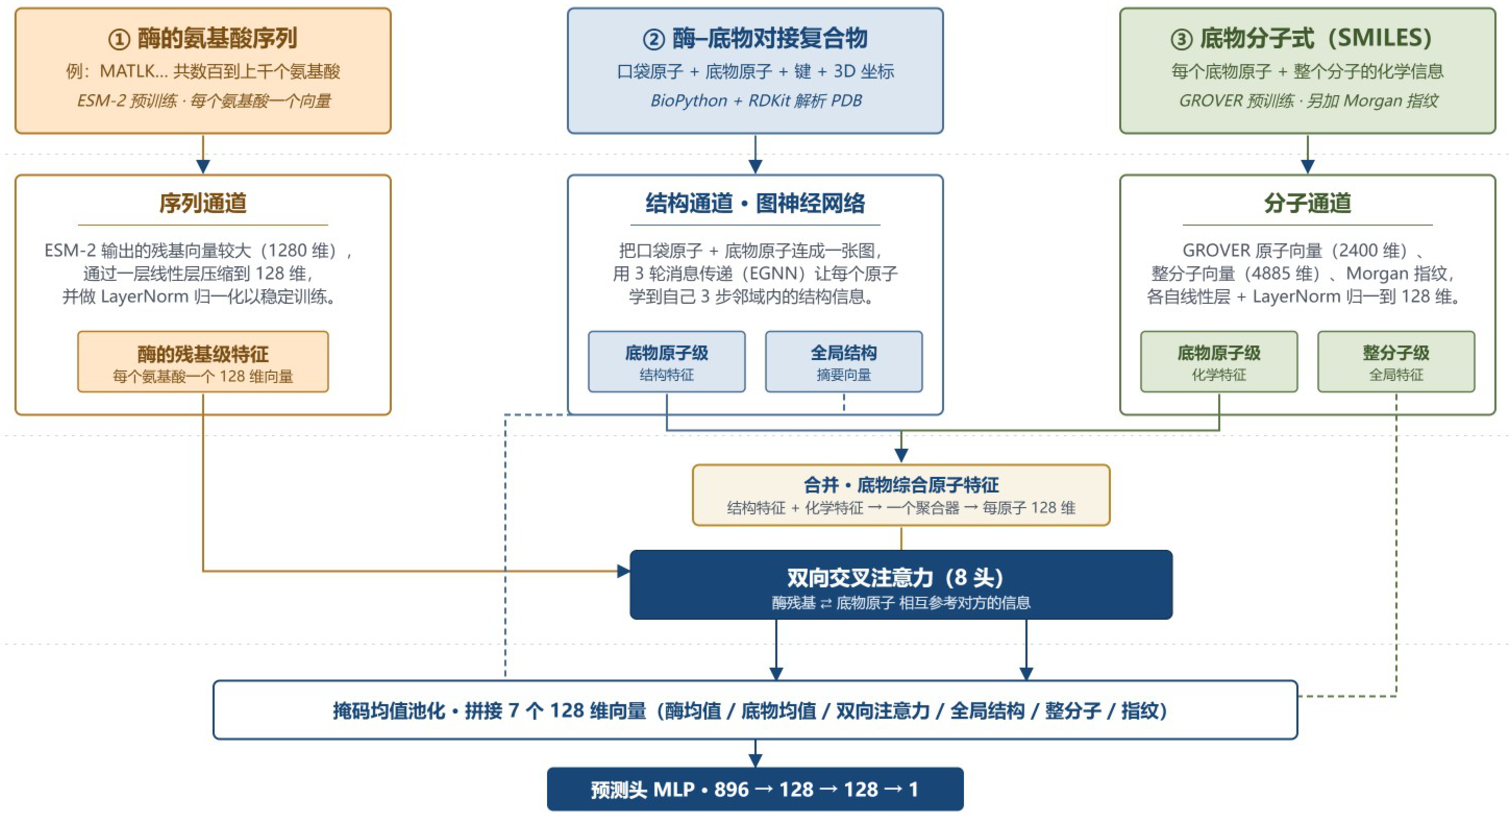
\includegraphics[width=1.25\textwidth]{./image/原始架构.pdf}}
  \caption{原架构 M0 总体示意：序列、结构与分子三通道并行编码，经双向交叉注意力使酶残基与底物原子互相参考，最终拼接 7 个 128 维向量送入预测头 MLP 输出二分类 logits}
  \label{fig:ch5-baseline}
\end{figure}

\section{双图架构设计动机与原理}
\label{sec:ch5-design}

\subsection{几何向量感知器（Geometric Vector Perceptron，GVP）}
\label{subsec:ch5-gvp}

GVP\cite{GVP2021} 是一类 SE(3)-等变（SE(3)-equivariant）层，区别于 SE(3)-不变层的根本特征在于：GVP 同时接受并输出两类表示——标量通道按常规神经网络方式变换，向量通道在空间旋转下"跟着转"。对整个口袋做整体旋转时，GVP 的标量输出保持不变，而向量输出以整体旋转矩阵作用后的新坐标给出。这一特性使 GVP 天然适合表达残基骨架朝向、侧链指向等方向依赖信息，而又不丢失原子级 EGNN 所依赖的距离关系。

基于上述考虑，本研究提出\textbf{双图架构}：在原架构保留原子级 EGNN 通路完全不变的基础上，新增一条残基级 GVP 通路与之并行运行。每个口袋残基被打包为一个节点，含"标量部分 + 向量部分"两组特征。\textbf{标量部分}用骨架主链二面角 $\varphi$、$\psi$、$\omega$ 的 $\sin$、$\cos$ 编码共 $6$ 维表达骨架的局部折叠构象；\textbf{向量部分}用 $\mathrm{C}\alpha \to \mathrm{N}$、$\mathrm{C}\alpha \to \mathrm{C}$、$\mathrm{C}\alpha \to \mathrm{C}\beta$ 三个三维方向向量共 $3 \times 3$ 维表达骨架朝向与侧链指向。残基节点之间的连边取每个残基空间最近邻 30 个残基，边特征含 $\mathrm{C}\alpha$--$\mathrm{C}\alpha$ 距离的径向基函数展开与 $\mathrm{C}\alpha$--$\mathrm{C}\alpha$ 方向向量。整个口袋旋转时 GVP 的标量输出不变、向量输出跟随旋转，几何关系被完整保留而不会被 SE(3)-不变所抛弃。

\subsection{双出口融合设计}
\label{subsec:ch5-fusion}

GVP 通路的输出（每残基 256 维，记为 $\mathbf{h}_{\mathrm{res}}$）通过两条独立路径注入主网络（见图~\ref{fig:ch5-arch}）。\emph{出口一（深融合）}将 $\mathbf{h}_{\mathrm{res}}$ 经线性层压至 128 维后按残基映射回注到序列通道的残基级特征之上，以更新双向交叉注意力\cite{Transformer2017} 的查询端；\emph{出口二（浅旁路）}将 $\mathbf{h}_{\mathrm{res}}$ 做残基均值池化压至 128 维，直接拼接入掩码池化后的综合向量。原架构在掩码池化后拼接的综合向量含 7 个 128 维分量（共 896 维），引入浅旁路后扩为 8 个分量（共 1024 维），随后送入多层感知机预测头输出二分类 logits。

\begin{figure}[!htbp]
  \centering
  \makebox[\textwidth][c]{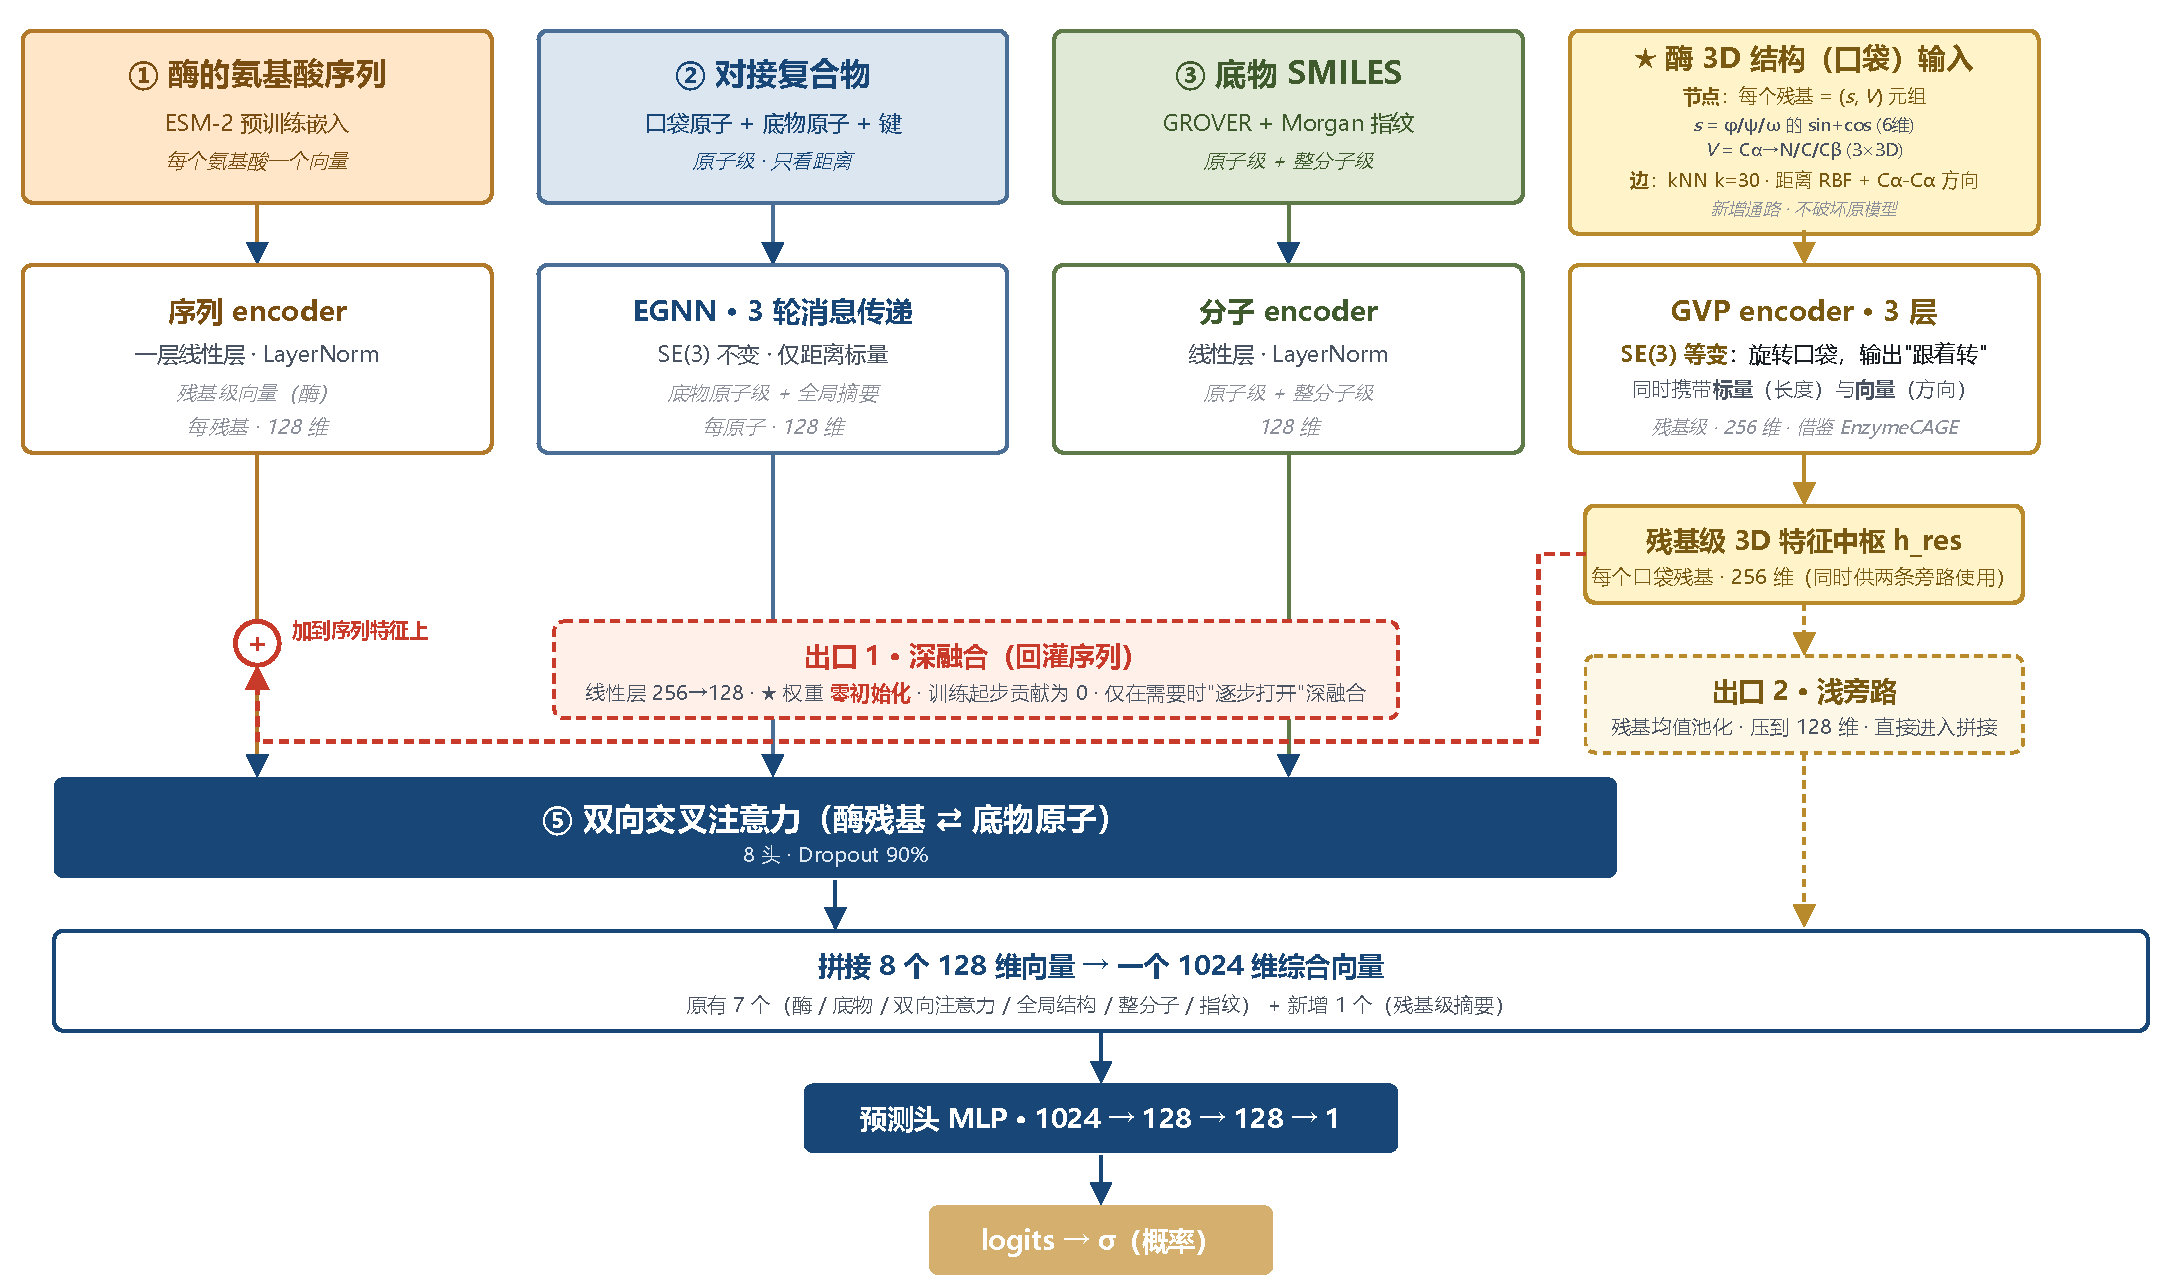
\includegraphics[width=1.25\textwidth]{./image/双图架构.pdf}}
  \caption{双图架构示意图：在原架构三通道基础上并行引入残基级 GVP 通路（右侧新增分支），输出经"出口一深融合"回灌序列通道、"出口二浅旁路"接入末端综合向量；零初始化与延迟解冻保证训练第 0 步与 M0 严格等价}
  \label{fig:ch5-arch}
\end{figure}

\section{残基级几何向量感知模块的实现}
\label{sec:ch5-implementation}

\subsection{GVP 编码器}
\label{subsec:ch5-encoder}

GVP 编码器由 3 层 GVP 构成，每层交替执行标量更新与向量更新，层间残差连接。实现上借鉴了公开的 GVP 参考实现\cite{GVP2021} 以及在酶--底物特异性任务上应用残基级 GVP 的 EnzymeCAGE 工程实现\cite{EnzymeCAGE2026}，并针对本研究的口袋数据规模（每口袋约 $30$--$100$ 个残基）调整了近邻半径与批处理策略。

\subsection{严格的基线等价性验证}
\label{subsec:ch5-equiv}

为避免双图架构在训练起步阶段对原架构 M0 的已有权重产生扰动，本研究对融合点做了\textbf{权重零初始化}：出口一深融合的线性层末层权重初始化为 $0$、出口二浅旁路在预测头中对应的新增 $128$ 维分量权重同样零初始化。在此设置下，模型第 0 步的前向输出严格等于原架构 M0，数值上最大绝对偏差为 $4 \times 10^{-8}$。这一验证确保了双图架构的效果差异只能来自训练过程中被梯度激活的 GVP 通路，而非初始化扰动。

\subsection{延迟解冻策略}
\label{subsec:ch5-unfreeze}

与零初始化配合，本研究采用延迟解冻：第 0 步时 GVP 分支所有参数梯度为 $0$、不参与权重更新；第 1 步起 GVP 分支被解冻并开始被梯度驱动。该设计使得训练起步与原架构完全一致、随即逐步激活新分支。由于第 0 步 GVP 分支存在参数但不参与反向传播，在分布式数据并行（Distributed Data Parallel，DDP）训练下需将 \texttt{find\_unused\_parameters} 设置为 \texttt{True} 以避免 PyTorch 的严格同步检查在首步报错；该选项引入约 5\%--10\% 的同步开销，但为延迟解冻设计所必需。

\subsection{规模与训练开销}
\label{subsec:ch5-scale}

双图架构相对原架构引入约 45\% 的新参数量（$1.85~\mathrm{M} \to 2.68~\mathrm{M}$），主要来自 GVP 编码器三层与出口融合线性层；每 epoch 训练时间由原架构的约 $55$ 秒增加至约 $60$ 秒，端到端训练成本增幅可控。

\section{双图架构训练与测试结果}
\label{sec:ch5-results}

双图架构模型 M1 的训练配置与第四章 \ref{sec:ch4-config} 节一致：4 块 RTX 5090 上 DDP 并行，单卡批大小 88、有效全局批大小 352，AdamW\cite{AdamW2019} 优化器，200 epoch 最大训练轮次，验证集 AUPR 为监控指标的早停机制。唯一变化在于 DDP 配置启用 \texttt{find\_unused\_parameters}。训练在第 57 个 epoch 早停，总耗时约 $56.8$ 分钟；验证集最佳 checkpoint 出现在第 $41$ 轮，对应 Val AUC $= 0.9262$。

在与原架构 M0 完全相同的随机切分第一折测试集（10{,}999 条样本、984 正 / 10{,}015 负）上评估 M1 的最佳 checkpoint，得到 \textbf{Test AUC $= 0.9310$、Test AUPR $= 0.6474$}。与原架构 M0（ep43，Test AUC $= 0.9302$、Test AUPR $= 0.6749$）的对比结果汇总于表~\ref{tab:ch5-results}。AUC 指标维度上，双图架构相对原架构观察到 $\Delta = +0.0008$ 的\textbf{微幅提升}；AUPR 指标维度上，双图架构相对原架构观察到 $\Delta = -0.0275$ 的\textbf{回落}。两项指标并列、对称报告，如实反映本研究的单折观察结果。

\begin{table}[htbp]
  \centering
  \caption{双模型在随机切分第一折测试集上的完整结果对比}
  \label{tab:ch5-results}
  \begin{tabular}{llcccc}
    \toprule
    模型 & 最佳 ckpt & Val AUC & Test AUC & Test AUPR & 参数量 \\
    \midrule
    原架构 M0      & ep43 & 0.9250 & 0.9302 & 0.6749 & 1.85 M \\
    双图架构 M1    & ep41 & 0.9262 & \textbf{0.9310} & 0.6474 & 2.68 M \\
    \midrule
    $\Delta$（M1 $-$ M0）  & --- & $+0.0012$ & $\bm{+0.0008}$ & $-0.0275$ & $+45\%$ \\
    \bottomrule
  \end{tabular}
\end{table}

\begin{figure}[!htbp]
  \centering
  \makebox[\textwidth][c]{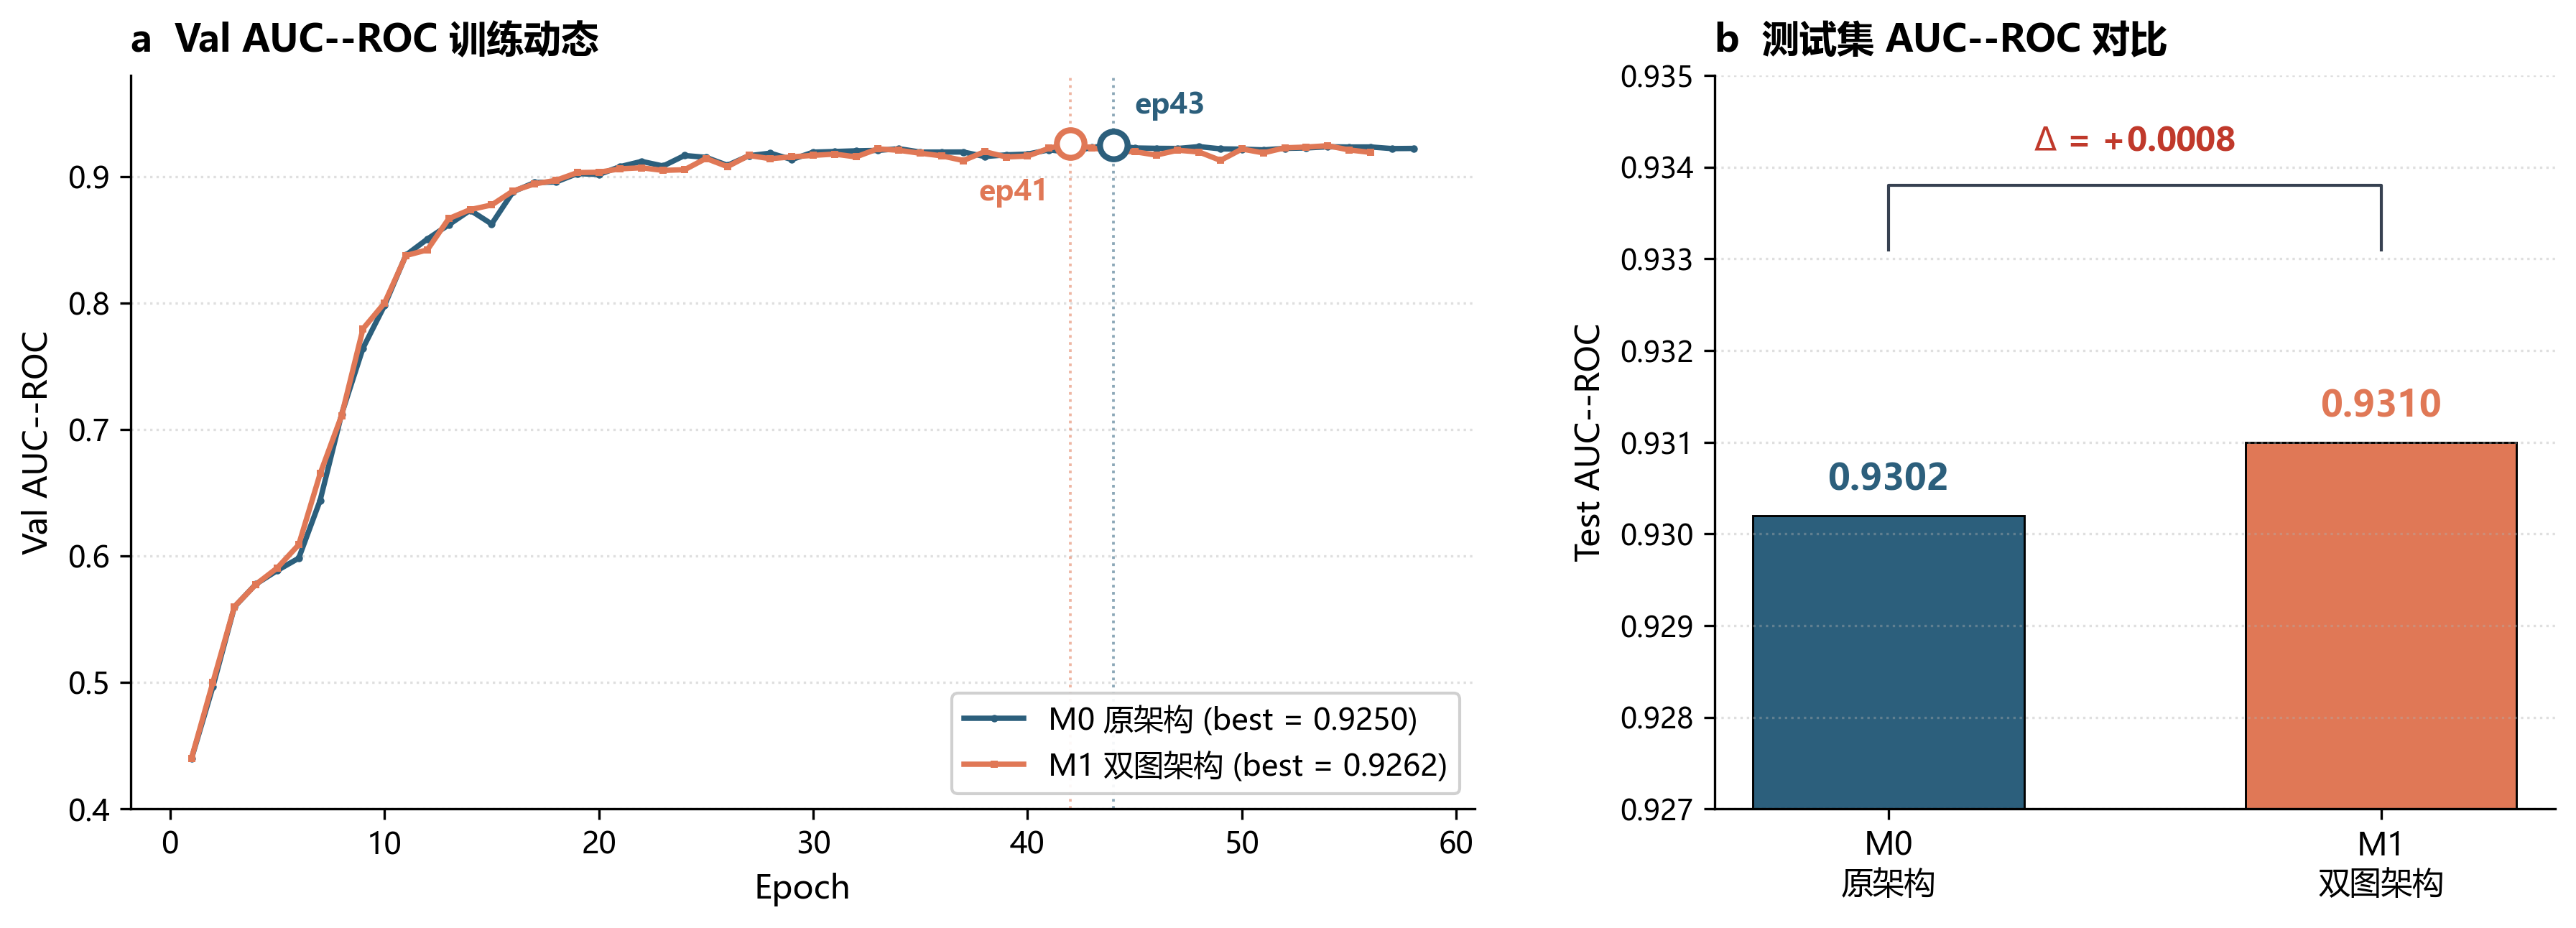
\includegraphics[width=1.15\textwidth]{./image/M0_M1对比.png}}
  \caption{原架构 M0 与双图架构 M1 对比：(a) Val AUC--ROC 训练曲线，M0 best ep43 = 0.9250，M1 best ep41 = 0.9262；(b) 测试集 AUC--ROC，M0 = 0.9302，M1 = 0.9310，$\Delta = +0.0008$}
  \label{fig:ch5-results}
\end{figure}

\section{结果讨论与方法学启示}
\label{sec:ch5-discussion}

\subsection{对单折观察的诚实解读}

上节表~\ref{tab:ch5-results} 给出的观察需要严格限定其有效范围。\textbf{AUC 微幅提升的方向}与第 \ref{sec:ch5-design} 节所述"对方向敏感的 P450 催化需要方向感知表征"物理假设方向一致，可作为双图架构\emph{架构工程层面}的初步可行性探索报告。然而，$+0.0008$ 的提升幅度处于单折评估的噪声边缘，加之训练时间（$56.8$ 分钟）与测试条件的唯一性，不足以支撑"双图架构在性能上优于原架构"的定性结论。\textbf{AUPR 的回落}同样需要诚实面对：$-0.0275$ 的下降在极不平衡数据（正负比约 $1:10$）上反映出模型对稀有正样本打分分布的扰动，其成因可能包括：未经充分超参调优情况下残基级通路导致的轻度过拟合、GVP 分支引入额外参数（$+45\%$）后在少数类上的优化困难、或单折评估本身的方差。本研究将此视为空间分辨率与优化难度之间的 trade-off 信号，不予强行淡化或选择性引用。

综合上述两点观察，本研究将双图架构定位为\textbf{对方向信息感知设计的初步可行性探索}，而非性能超越或稳健性结论。真正的稳健性判定需建立在多随机种子 $\times$ 多折交叉验证 $\times$ 充分超参调优 $\times$ 显著性检验的基础上，这些工作因单折的时间与资源限制未在本论文中完成，作为主要局限在第六章标注。

\subsection{对未来 P450 几何感知模型设计的启示}

上述受控单次观察仍对未来方法学设计提供了若干可操作的启示。第一，\textbf{方向感知通路作为距离感知通路的补充}具有进一步探索的价值：GVP 类模块在 P450 类几何敏感酶家族上虽然在本单折评估中未展现稳健的性能提升，但 AUC 方向与物理直觉一致，提示该方向值得以多折稳健评估为前提继续试验。第二，\textbf{标量--向量联合建模的工程可行性}已在本研究被验证：零初始化与延迟解冻的组合设计使得新分支可以在不破坏已有基线能力的前提下被逐步激活，该模式可推广到其他"在已训练好架构上加通路"的改进场景。第三，\textbf{极不平衡分类任务上的指标选择}不可仅依赖单一 AUC：本研究观察到的 AUC 提升与 AUPR 回落反向变化清楚说明，在正负比 $1:10$ 量级的任务上若仅报告 AUC 将遗漏对稀有正样本真实表现的关键信息；AUC 与 AUPR 并列评估应成为此类任务的默认做法\cite{Saito2015}。

本章的最终定位是：在第四章数据集层面与评估协议层面已确立的核心贡献之外，以架构工程角度补充一条带有方向感知能力的技术路线；所报告的数值观察与讨论均限定在单一随机折评估范围内，作为后续稳健性验证的起点而非终点。

%%
% 第六章 结论与展望
% 短且克制。四点创新 + 局限性如实声明 + 未来工作仅限方法学与数据层面。
%%

\chapter{结论与展望}
\label{cha:conclusion}

\section{主要结论与创新贡献}
\label{sec:contributions}

本论文以 \textit{Nature}~2025 发表的酶底物特异性预测 SOTA 模型 EZSpecificity\cite{EZSpec2025} 为参照框架，以其训练数据集 ESIBank 中覆盖显著稀缺（$389/25{,}225 \approx 1.5\%$）但应用价值极高的细胞色素 P450 超家族为试金石，系统检验了通用 SOTA 模型在稀缺家族上的 对未见酶的泛化能力，并在领域专属数据上开展重训与架构改进。综合全文工作，本研究的主要结论与创新贡献可归纳为以下四点。

\subsection{构建了目前规模最大、标注最详细的 P450 酶--底物特异性公开基准数据集}
\label{subsec:contrib-dataset}

现有 P450 数据库存在普遍局限：RCSB PDB\cite{Burley2025,Berman2000} 中共结晶配体可能是底物、产物、抑制剂或辅因子，未经区分直接使用会引入大量假阳性；ESIBank\cite{EZSpec2025} 基于 EC 号粗筛导致 FAD 单加氧酶等非 P450 混入；P450Rdb 的 132{,}000 条原始记录实为两表拼接，仅 3{,}753 条为实验验证条目；PlantP450DB\cite{Nelson2004} 与 PCPD\cite{Wang2021PCPD} 大量条目仅含酶序列与笼统反应描述而无标准化底物 SMILES。针对上述局限，本研究通过文献检索（PubMed + CrossRef）、PDB 结构分析（Fe--配体距离、配位关系、修饰特征）与多轮人工审核（辅以多智能体协作流程对每条酶--配体记录证据复核）严格区分底物、产物、抑制剂、辅因子与溶剂类型，整合得到 $1{,}622$ 个唯一酶、$2{,}125$ 个唯一底物、$4{,}751$ 条跨源去重正样本对、$47{,}510$ 条可用训练评估样本；相比 ESIBank 原始训练集在 P450 上的覆盖规模扩大约 4 倍，并显著扩展了植物 P450 的数据覆盖（PlantP450DB 与 PCPD 合计贡献 $2{,}188$ 条正样本与 $1{,}396$ 个唯一酶）。该基准数据集与对应的证据复核流程为后续社群验证、扩展与湿实验选样提供了可复用的基础设施。

\subsection{建立了一套泄漏控制的外部公平对比评估协议}
\label{subsec:contrib-protocol}

针对 SOTA 模型外部评估中训练集--测试集酶重合引发的记忆效应问题，本研究以 InterPro\cite{Blum2025} 功能域对 ESIBank 原始 $25{,}225$ 条酶严格识别出 $389$ 个真正的 P450，并据此从本研究测试集中剔除与之重合的 $3{,}036$ 条样本，得到 $7{,}963$ 条过滤后外部测试集。该协议将通用模型在 P450 上的评估条件收敛为"完全未见过的 P450 酶"，是对 SOTA 通用性声明在稀缺家族上进行严格检验的必要前提。

\subsection{实证发现 SOTA 通用模型在数据缺乏家族上存在未见酶的泛化瓶颈、领域专属重训可显著突破该瓶颈}
\label{subsec:contrib-finding}

在过滤后外部测试集（$n=7{,}963$）上：EZSpecificity 公开 checkpoint 仅取得 Test AUC $= 0.5586$、Test AUPR $= 0.1004$，AUPR 接近样本正负比下的随机基线；本研究在相同架构与领域专属数据上从头训练得到的基线模型 M0 达到 Test AUC $= 0.9205$、Test AUPR $= 0.6403$，相对参考模型的差距为 $\Delta\mathrm{AUC} = +0.3619$ 与 $\Delta\mathrm{AUPR} = +0.5399$。这一经验观察为"面向训练集稀缺家族的领域专属数据微调是必要的"这一方法学命题提供了量化支撑。

\subsection{提出并实现了面向方向信息感知的双图架构改进，并在单 fold 评估下展现了初步可行性}
\label{subsec:contrib-arch}

在原架构的原子级 EGNN 通路之外，本研究新增了一条残基级几何向量感知（GVP）通路，通过残基骨架二面角标量与 $\mathrm{C}\alpha \to \mathrm{N/C/C}\beta$ 向量联合编码捕获 SE(3)-等变的方向信息，并以零初始化 $+$ 延迟解冻的融合设计保证训练起步时对基线的严格等价（第 0 步数值最大绝对偏差 $4 \times 10^{-8}$）。在单 random fold 评估下，于未过滤测试集（$n=10{,}999$）上：双图架构 M1 相对原架构 M0 观察到 Test AUC $0.9302 \to 0.9310$ 的微幅提升（$\Delta = +0.0008$），同时 Test AUPR 由 $0.6749$ 回落至 $0.6474$（$\Delta = -0.0275$），两项指标并列对称报告。该观察作为方向信息感知设计的初步可行性探索，不作为性能超越或稳健性结论。

\subsection{研究意义与作用}
\label{subsec:contrib-impact}

本研究为 P450 底物特异性预测提供了可供社群验证与扩展的领域专属基准与泄漏控制评估协议，示范了在进行家族专属深度学习模型评估时泄漏控制的重要性；所提双图架构改进方案为后续在 P450 领域探索几何感知模型设计提供了可行的技术路线。研究结果对药学中 P450 代谢筛选工具的可信度评估、以及合成生物学中植物 P450 选择的辅助决策具有方法学参考意义。

\section{局限性}
\label{sec:limitations-final}

本研究的结论均严格限定于以下若干可审计的实验范围，相应局限在此集中声明。

\subsection{仅在单一随机切分上完成训练与评估}
\label{subsec:limit-fold}

本研究全部训练与测试结果均基于 random split 第一折，未开展 $k$ 折交叉验证、多随机种子重复或置信区间估计。因此第四章 $+0.3619$ AUC 差值与第五章 $+0.0008$ AUC 差值的稳健性范围未被系统量化。

\subsection{结构增强的观察不足以支撑稳健性断言}
\label{subsec:limit-structure}

双图架构 M1 的 AUC 微幅提升（$+0.0008$）处于单 fold 评估的噪声边缘，且 Test AUPR 同步出现 $-0.0275$ 的回落。本论文如实并列报告两项变化，将其定位为架构工程层面的初步可行性探索，不作为性能改进或机制结论；稳健性需待多 fold $\times$ 多 seed $\times$ 超参充分调优 $\times$ 显著性检验的系统评估。

\subsection{负样本基于随机配对假设}
\label{subsec:limit-neg}

本研究遵循 EZSpecificity 的双向随机负样本构造策略，假设在本研究样本空间中随机配对的酶--底物对以高概率为非催化关系。P450 家族内酶之间的序列与结构相似性较高，随机负样本中可能混入未被记录的真实正配对，引入假阴性；同家族难负样本的受控构造与评估未在本论文中系统开展。

\subsection{外部泄漏过滤仅限于酶层面}
\label{subsec:limit-leak}

本研究的过滤协议剔除了与 ESIBank 原始训练集中 $389$ 个 P450 酶重合的测试样本，但未进一步过滤底物层面与 ESIBank 训练集重合的部分；若某些底物作为 ESIBank 训练集中其他家族酶的底物出现过，其表征分布对参考模型可能仍具有一定熟悉性。

\subsection{对接姿态噪声与结构特征的不确定性}
\label{subsec:limit-dock}

对接姿态与真实结合构象之间存在不可避免的误差，结构通道的输入质量因此存在天然上限。AlphaFill 回填血红素的预测结构与晶体结构在活性位点细节上的一致性未做逐条评估。

\section{未来改进方向}
\label{sec:future-work}

本研究为 P450 底物特异性预测提供了数据、评估与架构三个层面的基础材料，后续工作可沿以下方法学与数据层面的方向展开。

\subsection{更严格的切分与稳健性评估}
\label{subsec:future-split}

在现有数据集上开展多随机切分 $+$ $k$ 折交叉验证 $+$ 多种子重复以建立稳健性置信区间；按酶的序列相似性聚类设计阶梯化测试集（例如限定测试与训练的序列一致度 $<40\%$），使评估难度梯度化并暴露模型在不同同源距离下的泛化曲线。

\subsection{困难负样本与评估协议的扩展}
\label{subsec:future-neg}

针对"同家族难负样本"单独构造可控测试集，系统度量模型在同家族内部区分不同酶--底物偏好的能力；将外部泄漏过滤从酶层面扩展到底物层面以进一步收紧公平对比条件。

\subsection{底物类别作为辅助监督信号}
\label{subsec:future-class}

本研究在数据清洗过程中已将 $2{,}125$ 个底物按 NPClassifier\cite{NPClassifier2021} 体系分为萜类、氨基酸、脂肪酸、生物碱、甾体、苯丙素、聚酮与其他共 $8$ 大类；未来可将底物类别作为辅助任务监督主模型的多任务训练，检验类别先验对 P450 特异性预测的帮助。

\subsection{双图架构的稳健性验证与拓展}
\label{subsec:future-arch}

在多 fold 稳健性评估框架下重做双图架构 M1 与原架构 M0 的对比，以确认本论文观察到的 $+0.0008$ AUC 提升与 $-0.0275$ AUPR 回落分别是否具有跨 fold 的一致性；在此基础上探索融合策略（深融合 vs 浅旁路权重）与 GVP 层数等超参的系统扫描。

\subsection{从二分类到区域选择性与反应级预测}
\label{subsec:future-reaction}

P450 的实际价值不仅在于判断酶--底物配对的是非，更在于预测催化后的产物结构与区域选择性；本研究数据集中的 PCPD 反应图片（$857$ 张）与 P450Rdb 反应 SMILES 可作为向反应级预测扩展的基础数据。

\subsection{可解释性与湿实验验证}
\label{subsec:future-validate}

在模型预测基础上做注意力热图与口袋--底物原子级贡献分析以辅助药学家解释；选择若干高置信度预测配对开展体外酶活实验或 KCAT/Km 测定以验证模型可靠性，并反馈用于模型迭代。


\bibliography{reference}  % 参考文献使用 BibTeX 编译
% \printbibliography       % 参考文献使用 BibLaTeX 编译

% \appendix
% % !TeX root = ../main.tex
%%
% 附录A 补充数据与脚本
% 按中山大学规范二（六）8 附录内容要求
%%

\chapter{补充数据与脚本}
\label{app:supplementary}

本附录汇总与正文互补的实现细节，包括各数据源的字段对照与获取参数、数据一致性校验协议的技术细节，以及基线与双图架构两模型的完整训练超参数表。

\section{数据源字段对照}
\label{app:data-sources}

本研究所采用的五个数据源在原始字段与获取通道上存在差异，表~\ref{tab:app-sources} 汇总了各源提供的核心字段、获取方式与关键过滤标准，以便后续社群复用。

\begin{table}[htbp]
  \centering
  \caption{五个数据源的核心字段与获取方式}
  \label{tab:app-sources}
  \begin{tabular}{llp{0.35\textwidth}l}
    \toprule
    来源 & 访问通道 & 关键字段与处理 & 代表性过滤 \\
    \midrule
    RCSB PDB & REST API / FTP      & UniProt 登录号、PDB ID、配体 CCD 码、分辨率、序列长度                               & 分辨率 $\leq 3.0~\mathrm{\AA}$；序列 300--1{,}200 aa \\
    ESIBank  & EZSpecificity 数据包 & 酶序列、反应 SMILES、正样本标签、索引                                              & 过滤 10 种辅因子与溶剂 \\
    P450Rdb  & 官网文件下载         & UniProt 登录号、反应描述、文献标签、实验证据等级                                     & Experimentally validated 条目 \\
    PlantP450DB & 爬虫 + 文献自动抽取 & 酶名、家族、物种、底物描述、文献 DOI                                                 & 需经 PubMed/CrossRef 文献补齐 \\
    PCPD     & CDN JSON 批量下载    & 酶 JSON、FASTA 序列、PDB 结构、反应示意图片                                          & 正则抽取 + 多智能体协作清洗 \\
    \bottomrule
  \end{tabular}
\end{table}

\section{数据一致性校验方法与脚本说明}
\label{app:qc-protocol}

本研究的数据一致性校验由两部分组成：索引对齐核验协议与多智能体协作证据判定的工具栈。

\subsection{索引对齐核验协议}
\label{subsec:qc-index}

LMDB 存储与原始 CSV 行号之间的对齐使用酶序列 SHA 哈希与底物规范化 SMILES 作为校验键，对全量样本进行往返比对。具体流程：首先按训练集、验证集、测试集分别读取切分索引文件中的 \texttt{(enzyme\_id, substrate\_id)} 对；然后从 LMDB 中读取对应的酶序列与底物 SMILES，计算 SHA-256 哈希与经 RDKit 规范化后的标准 SMILES；再与原始 \texttt{Enzymes.csv} 与 \texttt{Substrates.csv} 中对应行号的字段做逐条比对，记录任何键值不一致的条目并写入 \texttt{qc\_report.csv}。初版流水线中识别出的索引错位问题经修复后，完整数据集通过全链路一致性核验。

\subsection{多智能体协作工具栈}
\label{subsec:qc-multiagent}

第 \ref{sec:multiagent} 节所述证据级联判定流程在 Claude Code 命令行环境下运行，外部的 OpenAI Codex 与 Google Gemini 模型通过模型上下文协议（Model Context Protocol，MCP）封装接入：Codex 侧通过 \texttt{codex-mcp} 开源组件、Gemini 侧通过 \texttt{gemini-mcp} 开源组件实现函数级调用。主代理（Claude）在每条判定任务上分别向文献代理（Gemini）与结构代理（Codex）派发独立查询，两代理相互不可见以避免证据耦合。在 12 个并行窗口上每条记录约 15 分钟的处理节奏下，RCSB 的 682 条 P450--配体配对约在 $57$ 条每窗口的负载下完成全量复核。

\section{训练超参数完整表}
\label{app:hyperparameters}

表~\ref{tab:app-hparams} 汇总了原架构基线模型 M0 与双图架构模型 M1 在本研究中的完整训练超参数。两模型的共享超参数保持完全一致以确保单变量消融，仅在与 GVP 分支相关的架构超参数与 DDP 的 \texttt{find\_unused\_parameters} 选项上存在差异。

\begin{table}[htbp]
  \centering
  \caption{两模型训练超参数对照}
  \label{tab:app-hparams}
  \begin{tabular}{lll}
    \toprule
    超参数项 & M0（原架构）& M1（双图架构）\\
    \midrule
    GPU 数量            & 4 $\times$ RTX 5090 & 4 $\times$ RTX 5090 \\
    并行策略            & DDP                  & DDP \\
    \texttt{find\_unused\_params} & False      & \textbf{True}（延迟解冻所需）\\
    单卡批大小          & 88                   & 88 \\
    有效全局批大小      & 352                  & 352 \\
    混合精度            & 启用                 & 启用 \\
    优化器              & AdamW                & AdamW \\
    初始学习率          & $5 \times 10^{-4}$   & $5 \times 10^{-4}$ \\
    权重衰减            & $1 \times 10^{-5}$   & $1 \times 10^{-5}$ \\
    $\beta_1$, $\beta_2$ & $0.9, 0.999$        & $0.9, 0.999$ \\
    学习率调度          & ReduceLROnPlateau    & ReduceLROnPlateau \\
    最大 epoch          & 200                  & 200 \\
    早停监控            & val AUPR             & val AUPR \\
    早停耐心            & 15 epoch             & 15 epoch \\
    损失函数            & 加权 BCEWithLogits   & 加权 BCEWithLogits \\
    \midrule
    隐藏维度            & 128                  & 128 \\
    EGNN 层数           & 3                    & 3 \\
    EGNN 近邻 $k$       & 48                   & 48 \\
    GVP 层数            & ---                  & 3 \\
    GVP 残基近邻 $k$    & ---                  & 30 \\
    残基标量维度        & ---                  & 6（$\varphi$、$\psi$、$\omega$ 的 $\sin/\cos$）\\
    残基向量维度        & ---                  & $3 \times 3$（$\mathrm{C}\alpha \to \mathrm{N}/\mathrm{C}/\mathrm{C}\beta$）\\
    交叉注意力头数      & 8                    & 8 \\
    注意力 dropout      & $0.9$                & $0.9$ \\
    预测头综合向量维度  & 896                  & 1024 \\
    参数量              & $\sim 1.85~\mathrm{M}$ & $\sim 2.68~\mathrm{M}$ \\
    \midrule
    训练实际 epoch      & 57（早停）           & 57（早停）\\
    最佳 checkpoint     & ep43                 & ep41 \\
    训练总耗时          & $\sim 56.8$ min      & $\sim 56.8$ min \\
    \bottomrule
  \end{tabular}
\end{table}

\section{其他内部探索实验}
\label{app:other-experiments}

除本论文正文报告的原架构基线（M0）与双图架构（M1）两组实验外，本研究团队在数据集构建与基础模型探索阶段曾开展若干内部诊断与结构特征增强实验，包括早期版本的 LMDB 索引对齐问题诊断复现与基于血红素铁原子编码、残基主链--侧链二面角扩维等方向的结构特征增强尝试。上述内部探索的测试结果因污染期数据或单变量显著性不充分而未纳入本论文的正式结果报告；相关原始日志与检查点保留于实验服务器归档目录，作为后续稳健性验证的基础参考。


\backmatter
% 盲审版：以下一行已注释，移除致谢
% % !TeX root = ../main.tex

\begin{acknowledgements}

    四年本科生活转眼即逝，从初入校园时的懵懂到今日完成这篇毕业论文，回首走过的路，所学远不止于课本中的知识与技能，更包括独立面对未知问题的方法、面对挫折时的耐心，以及科研工作所必需的求实与诚实。一段段成长的背后，离不开师长的悉心指导、朋友的相互扶持与家人的默默守候，谨借这一隅篇幅，向他们郑重致谢。

    首先要感谢我的指导老师王家祺老师。在课题选择、思路搭建、实验执行与论文写作的每一个阶段，王老师都给予了清晰而精准的指导。每当我陷入细节的纠缠，他总能以更高的视角点出问题的关键，让我得以从局部跳出、回到主线；每当我对结果的解释失之过度时，他又会及时提醒我对数据保持敬畏、对结论保持克制。他严谨求实的治学态度、对学生独立思考的尊重、以及在繁忙工作中仍坚持逐字逐句审阅论文的耐心，都是我科研生涯起点处最珍贵的榜样。在此谨向王老师致以崇高的敬意与最诚挚的感谢。

    申请季那段焦灼难捱的日子里，要感谢中山大学电子与通信工程学院的刘瀚文同学始终与我同行。我们在彼此的不确定中相互托底，把许多原本难以独自消化的压力分担成了两个人的从容。这份在最不轻松的时节里仍愿意并肩的友谊，是我本科四年最幸运的相遇之一。

    最后，要把最深的感谢留给我的家人。父母用日复一日的辛劳支撑起我无忧的求学条件，更用言传身教教会我何为正直、何为坚持；每当我面对选择犹豫不决，他们总是耐心倾听、给出最中肯的建议，又在我决定之后给予最坚定的支持。也要感谢我的哥哥，作为同样走过这条路的过来人，他在许多关键节点上给了我最踏实的提醒与陪伴，让我在前行时多了一份从容。这份家人的恩情远非言语可以承载，唯愿在未来的日子里以更踏实的脚步去回报。

    谨以此文，献给所有曾在这段旅程中给予我帮助与陪伴的人。

\end{acknowledgements}

% 本科期间无与毕业论文相关的已发表科研成果，按规范二（八）省略"相关科研成果目录"
% \input{docs/achievements.tex}

\end{document}
